\documentclass[1p]{elsarticle_modified}
%\bibliographystyle{elsarticle-num}

%\usepackage[colorlinks]{hyperref}
%\usepackage{abbrmath_seonhwa} %\Abb, \Ascr, \Acal ,\Abf, \Afrak
\usepackage{amsfonts}
\usepackage{amssymb}
\usepackage{amsmath}
\usepackage{amsthm}
\usepackage{scalefnt}
\usepackage{amsbsy}
\usepackage{kotex}
\usepackage{caption}
\usepackage{subfig}
\usepackage{color}
\usepackage{graphicx}
\usepackage{xcolor} %% white, black, red, green, blue, cyan, magenta, yellow
\usepackage{float}
\usepackage{setspace}
\usepackage{hyperref}

\usepackage{tikz}
\usetikzlibrary{arrows}

\usepackage{multirow}
\usepackage{array} % fixed length table
\usepackage{hhline}

%%%%%%%%%%%%%%%%%%%%%
\makeatletter
\renewcommand*\env@matrix[1][\arraystretch]{%
	\edef\arraystretch{#1}%
	\hskip -\arraycolsep
	\let\@ifnextchar\new@ifnextchar
	\array{*\c@MaxMatrixCols c}}
\makeatother %https://tex.stackexchange.com/questions/14071/how-can-i-increase-the-line-spacing-in-a-matrix
%%%%%%%%%%%%%%%

\usepackage[normalem]{ulem}

\newcommand{\msout}[1]{\ifmmode\text{\sout{\ensuremath{#1}}}\else\sout{#1}\fi}
%SOURCE: \msout is \stkout macro in https://tex.stackexchange.com/questions/20609/strikeout-in-math-mode

\newcommand{\cancel}[1]{
	\ifmmode
	{\color{red}\msout{#1}}
	\else
	{\color{red}\sout{#1}}
	\fi
}

\newcommand{\add}[1]{
	{\color{blue}\uwave{#1}}
}

\newcommand{\replace}[2]{
	\ifmmode
	{\color{red}\msout{#1}}{\color{blue}\uwave{#2}}
	\else
	{\color{red}\sout{#1}}{\color{blue}\uwave{#2}}
	\fi
}

\newcommand{\Sol}{\mathcal{S}} %segment
\newcommand{\D}{D} %diagram
\newcommand{\A}{\mathcal{A}} %arc


%%%%%%%%%%%%%%%%%%%%%%%%%%%%%5 test

\def\sl{\operatorname{\textup{SL}}(2,\Cbb)}
\def\psl{\operatorname{\textup{PSL}}(2,\Cbb)}
\def\quan{\mkern 1mu \triangleright \mkern 1mu}

\theoremstyle{definition}
\newtheorem{thm}{Theorem}[section]
\newtheorem{prop}[thm]{Proposition}
\newtheorem{lem}[thm]{Lemma}
\newtheorem{ques}[thm]{Question}
\newtheorem{cor}[thm]{Corollary}
\newtheorem{defn}[thm]{Definition}
\newtheorem{exam}[thm]{Example}
\newtheorem{rmk}[thm]{Remark}
\newtheorem{alg}[thm]{Algorithm}

\newcommand{\I}{\sqrt{-1}}
\begin{document}

%\begin{frontmatter}
%
%\title{Boundary parabolic representations of knots up to 8 crossings}
%
%%% Group authors per affiliation:
%\author{Yunhi Cho} 
%\address{Department of Mathematics, University of Seoul, Seoul, Korea}
%\ead{yhcho@uos.ac.kr}
%
%
%\author{Seonhwa Kim} %\fnref{s_kim}}
%\address{Center for Geometry and Physics, Institute for Basic Science, Pohang, 37673, Korea}
%\ead{ryeona17@ibs.re.kr}
%
%\author{Hyuk Kim}
%\address{Department of Mathematical Sciences, Seoul National University, Seoul 08826, Korea}
%\ead{hyukkim@snu.ac.kr}
%
%\author{Seokbeom Yoon}
%\address{Department of Mathematical Sciences, Seoul National University, Seoul, 08826,  Korea}
%\ead{sbyoon15@snu.ac.kr}
%
%\begin{abstract}
%We find all boundary parabolic representation of knots up to 8 crossings.
%
%\end{abstract}
%\begin{keyword}
%    \MSC[2010] 57M25 
%\end{keyword}
%
%\end{frontmatter}

%\linenumbers
%\tableofcontents
%
\newcommand\colored[1]{\textcolor{white}{\rule[-0.35ex]{0.8em}{1.4ex}}\kern-0.8em\color{red} #1}%
%\newcommand\colored[1]{\textcolor{white}{ #1}\kern-2.17ex	\textcolor{white}{ #1}\kern-1.81ex	\textcolor{white}{ #1}\kern-2.15ex\color{red}#1	}

{\Large $\underline{12a_{0358}~(K12a_{0358})}$}

\setlength{\tabcolsep}{10pt}
\renewcommand{\arraystretch}{1.6}
\vspace{1cm}\begin{tabular}{m{100pt}>{\centering\arraybackslash}m{274pt}}
\multirow{5}{120pt}{
	\centering
	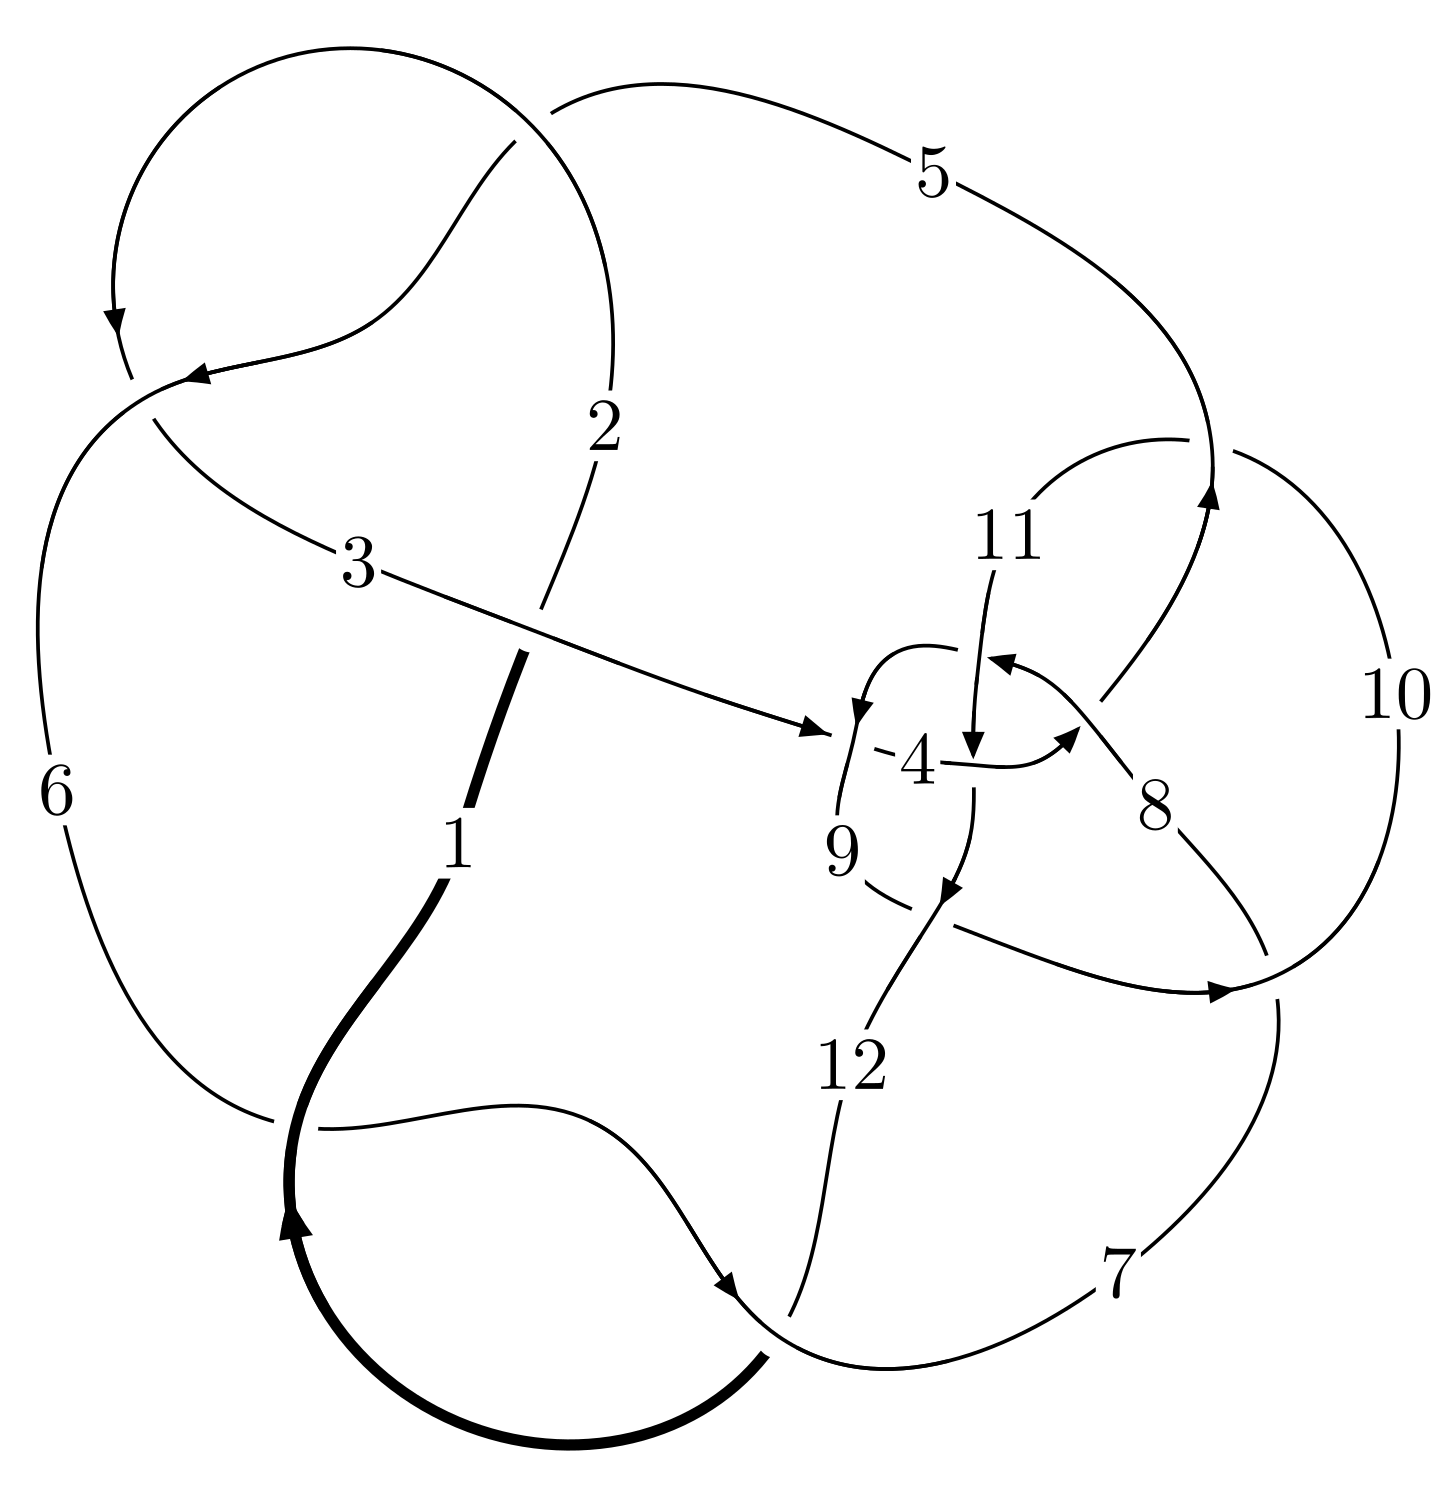
\includegraphics[width=112pt]{../../../GIT/diagram.site/Diagrams/png/1159_12a_0358.png}\\
\ \ \ A knot diagram\footnotemark}&
\allowdisplaybreaks
\textbf{Linearized knot diagam} \\
\cline{2-2}
 &
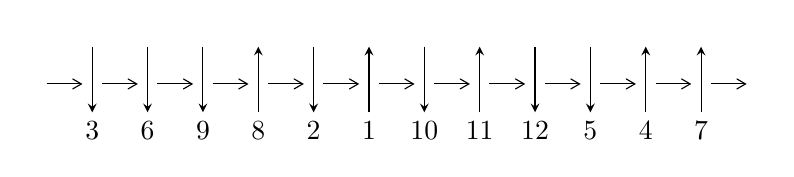
\begin{tikzpicture}[x=20pt, y=17pt]
	% nodes
	\node (C0) at (0, 0) {};
	\node (C1) at (1, 0) {};
	\node (C1U) at (1, +1) {};
	\node (C1D) at (1, -1) {3};

	\node (C2) at (2, 0) {};
	\node (C2U) at (2, +1) {};
	\node (C2D) at (2, -1) {6};

	\node (C3) at (3, 0) {};
	\node (C3U) at (3, +1) {};
	\node (C3D) at (3, -1) {9};

	\node (C4) at (4, 0) {};
	\node (C4U) at (4, +1) {};
	\node (C4D) at (4, -1) {8};

	\node (C5) at (5, 0) {};
	\node (C5U) at (5, +1) {};
	\node (C5D) at (5, -1) {2};

	\node (C6) at (6, 0) {};
	\node (C6U) at (6, +1) {};
	\node (C6D) at (6, -1) {1};

	\node (C7) at (7, 0) {};
	\node (C7U) at (7, +1) {};
	\node (C7D) at (7, -1) {10};

	\node (C8) at (8, 0) {};
	\node (C8U) at (8, +1) {};
	\node (C8D) at (8, -1) {11};

	\node (C9) at (9, 0) {};
	\node (C9U) at (9, +1) {};
	\node (C9D) at (9, -1) {12};

	\node (C10) at (10, 0) {};
	\node (C10U) at (10, +1) {};
	\node (C10D) at (10, -1) {5};

	\node (C11) at (11, 0) {};
	\node (C11U) at (11, +1) {};
	\node (C11D) at (11, -1) {4};

	\node (C12) at (12, 0) {};
	\node (C12U) at (12, +1) {};
	\node (C12D) at (12, -1) {7};
	\node (C13) at (13, 0) {};

	% arrows
	\draw[->,>={angle 60}]
	(C0) edge (C1) (C1) edge (C2) (C2) edge (C3) (C3) edge (C4) (C4) edge (C5) (C5) edge (C6) (C6) edge (C7) (C7) edge (C8) (C8) edge (C9) (C9) edge (C10) (C10) edge (C11) (C11) edge (C12) (C12) edge (C13) ;	\draw[->,>=stealth]
	(C1U) edge (C1D) (C2U) edge (C2D) (C3U) edge (C3D) (C4D) edge (C4U) (C5U) edge (C5D) (C6D) edge (C6U) (C7U) edge (C7D) (C8D) edge (C8U) (C9U) edge (C9D) (C10U) edge (C10D) (C11D) edge (C11U) (C12D) edge (C12U) ;
	\end{tikzpicture} \\
\hhline{~~} \\& 
\textbf{Solving Sequence} \\ \cline{2-2} 
 &
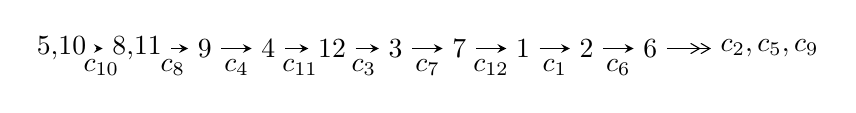
\begin{tikzpicture}[x=23pt, y=7pt]
	% node
	\node (A0) at (-1/8, 0) {5,10};
	\node (A1) at (17/16, 0) {8,11};
	\node (A2) at (17/8, 0) {9};
	\node (A3) at (25/8, 0) {4};
	\node (A4) at (33/8, 0) {12};
	\node (A5) at (41/8, 0) {3};
	\node (A6) at (49/8, 0) {7};
	\node (A7) at (57/8, 0) {1};
	\node (A8) at (65/8, 0) {2};
	\node (A9) at (73/8, 0) {6};
	\node (C1) at (1/2, -1) {$c_{10}$};
	\node (C2) at (13/8, -1) {$c_{8}$};
	\node (C3) at (21/8, -1) {$c_{4}$};
	\node (C4) at (29/8, -1) {$c_{11}$};
	\node (C5) at (37/8, -1) {$c_{3}$};
	\node (C6) at (45/8, -1) {$c_{7}$};
	\node (C7) at (53/8, -1) {$c_{12}$};
	\node (C8) at (61/8, -1) {$c_{1}$};
	\node (C9) at (69/8, -1) {$c_{6}$};
	\node (A10) at (11, 0) {$c_{2},c_{5},c_{9}$};

	% edge
	\draw[->,>=stealth]	
	(A0) edge (A1) (A1) edge (A2) (A2) edge (A3) (A3) edge (A4) (A4) edge (A5) (A5) edge (A6) (A6) edge (A7) (A7) edge (A8) (A8) edge (A9) ;
	\draw[->>,>={angle 60}]	
	(A9) edge (A10);
\end{tikzpicture} \\ 

\end{tabular} \\

\footnotetext{
The image of knot diagram is generated by the software ``\textbf{Draw programme}" developed by Andrew Bartholomew(\url{http://www.layer8.co.uk/maths/draw/index.htm\#Running-draw}), where we modified some parts for our purpose(\url{https://github.com/CATsTAILs/LinksPainter}).
}\phantom \\ \newline 
\centering \textbf{Ideals for irreducible components\footnotemark of $X_{\text{par}}$} 
 
\begin{align*}
I^u_{1}&=\langle 
-3.48000\times10^{182} u^{67}+2.10373\times10^{182} u^{66}+\cdots+2.76730\times10^{181} b-5.41435\times10^{182},\\
\phantom{I^u_{1}}&\phantom{= \langle  }-2.95579\times10^{182} u^{67}+4.27734\times10^{182} u^{66}+\cdots+2.76730\times10^{181} a-3.31608\times10^{183},\\
\phantom{I^u_{1}}&\phantom{= \langle  }u^{68}+19 u^{64}+\cdots-7 u+1\rangle \\
I^u_{2}&=\langle 
1.53296\times10^{479} u^{85}+3.33392\times10^{478} u^{84}+\cdots+2.77033\times10^{479} b+4.69150\times10^{478},\\
\phantom{I^u_{2}}&\phantom{= \langle  }1.19862\times10^{480} u^{85}+1.80990\times10^{479} u^{84}+\cdots+2.77033\times10^{479} a+4.42171\times10^{479},\;u^{86}-4 u^{84}+\cdots+43 u-1\rangle \\
I^u_{3}&=\langle 
u^2+b,\;u^{24}+u^{23}+\cdots+a+6,\;u^{25}-4 u^{23}+\cdots+u-1\rangle \\
I^u_{4}&=\langle 
b+1,\;a- u,\;u^2- u+1\rangle \\
\\
\end{align*}
\raggedright * 4 irreducible components of $\dim_{\mathbb{C}}=0$, with total 181 representations.\\
\footnotetext{All coefficients of polynomials are rational numbers. But the coefficients are sometimes approximated in decimal forms when there is not enough margin.}
\newpage
\renewcommand{\arraystretch}{1}
\centering \section*{I. $I^u_{1}= \langle -3.48\times10^{182} u^{67}+2.10\times10^{182} u^{66}+\cdots+2.77\times10^{181} b-5.41\times10^{182},\;-2.96\times10^{182} u^{67}+4.28\times10^{182} u^{66}+\cdots+2.77\times10^{181} a-3.32\times10^{183},\;u^{68}+19 u^{64}+\cdots-7 u+1 \rangle$}
\flushleft \textbf{(i) Arc colorings}\\
\begin{tabular}{m{7pt} m{180pt} m{7pt} m{180pt} }
\flushright $a_{5}=$&$\begin{pmatrix}0\\u\end{pmatrix}$ \\
\flushright $a_{10}=$&$\begin{pmatrix}1\\0\end{pmatrix}$ \\
\flushright $a_{8}=$&$\begin{pmatrix}10.6811 u^{67}-15.4567 u^{66}+\cdots-497.371 u+119.831\\12.5754 u^{67}-7.60209 u^{66}+\cdots-175.533 u+19.5654\end{pmatrix}$ \\
\flushright $a_{11}=$&$\begin{pmatrix}1\\u^2\end{pmatrix}$ \\
\flushright $a_{9}=$&$\begin{pmatrix}17.7268 u^{67}-20.5532 u^{66}+\cdots-554.027 u+123.940\\16.3036 u^{67}-10.0984 u^{66}+\cdots-218.254 u+24.6619\end{pmatrix}$ \\
\flushright $a_{4}=$&$\begin{pmatrix}29.9768 u^{67}-19.8927 u^{66}+\cdots-442.656 u+71.3591\\-3.63379 u^{67}-1.04843 u^{66}+\cdots+25.3732 u+9.21156\end{pmatrix}$ \\
\flushright $a_{12}=$&$\begin{pmatrix}32.7837 u^{67}-10.4113 u^{66}+\cdots-206.024 u-32.1867\\-12.5754 u^{67}+7.60209 u^{66}+\cdots+175.533 u-19.5654\end{pmatrix}$ \\
\flushright $a_{3}=$&$\begin{pmatrix}9.42361 u^{67}-10.6348 u^{66}+\cdots-194.629 u+53.6323\\-13.7322 u^{67}+4.68970 u^{66}+\cdots+164.160 u-7.09202\end{pmatrix}$ \\
\flushright $a_{7}=$&$\begin{pmatrix}23.2565 u^{67}-23.0588 u^{66}+\cdots-672.905 u+139.396\\12.5754 u^{67}-7.60209 u^{66}+\cdots-175.533 u+19.5654\end{pmatrix}$ \\
\flushright $a_{1}=$&$\begin{pmatrix}15.3311 u^{67}-11.3111 u^{66}+\cdots-106.397 u+4.70936\\-11.6073 u^{67}+5.60830 u^{66}+\cdots+231.455 u-30.3761\end{pmatrix}$ \\
\flushright $a_{2}=$&$\begin{pmatrix}15.8016 u^{67}-18.6094 u^{66}+\cdots-268.617 u+59.5037\\15.4207 u^{67}-9.11330 u^{66}+\cdots-110.867 u+3.78552\end{pmatrix}$ \\
\flushright $a_{6}=$&$\begin{pmatrix}-20.4648 u^{67}+7.34855 u^{66}+\cdots-44.9005 u+53.2777\\-1.24532 u^{67}+3.69828 u^{66}+\cdots-32.5923 u-1.47535\end{pmatrix}$\\&\end{tabular}
\flushleft \textbf{(ii) Obstruction class $= -1$}\\~\\
\flushleft \textbf{(iii) Cusp Shapes $= 116.467 u^{67}-60.5514 u^{66}+\cdots-1629.96 u+139.411$}\\~\\
\newpage\renewcommand{\arraystretch}{1}
\flushleft \textbf{(iv) u-Polynomials at the component}\newline \\
\begin{tabular}{m{50pt}|m{274pt}}
Crossings & \hspace{64pt}u-Polynomials at each crossing \\
\hline $$\begin{aligned}c_{1}\end{aligned}$$&$\begin{aligned}
&u^{68}+37 u^{67}+\cdots+89 u+16
\end{aligned}$\\
\hline $$\begin{aligned}c_{2},c_{5}\end{aligned}$$&$\begin{aligned}
&u^{68}+5 u^{67}+\cdots+33 u+4
\end{aligned}$\\
\hline $$\begin{aligned}c_{3},c_{10}\end{aligned}$$&$\begin{aligned}
&u^{68}+19 u^{64}+\cdots-7 u+1
\end{aligned}$\\
\hline $$\begin{aligned}c_{4},c_{11}\end{aligned}$$&$\begin{aligned}
&u^{68}- u^{67}+\cdots+36 u^2+1
\end{aligned}$\\
\hline $$\begin{aligned}c_{6},c_{12}\end{aligned}$$&$\begin{aligned}
&u^{68}+15 u^{67}+\cdots+233 u+4
\end{aligned}$\\
\hline $$\begin{aligned}c_{7},c_{9}\end{aligned}$$&$\begin{aligned}
&u^{68}+10 u^{67}+\cdots-27 u+1
\end{aligned}$\\
\hline $$\begin{aligned}c_{8}\end{aligned}$$&$\begin{aligned}
&u^{68}+38 u^{67}+\cdots+17 u+2
\end{aligned}$\\
\hline
\end{tabular}\\~\\
\newpage\renewcommand{\arraystretch}{1}
\flushleft \textbf{(v) Riley Polynomials at the component}\newline \\
\begin{tabular}{m{50pt}|m{274pt}}
Crossings & \hspace{64pt}Riley Polynomials at each crossing \\
\hline $$\begin{aligned}c_{1}\end{aligned}$$&$\begin{aligned}
&y^{68}-9 y^{67}+\cdots+2287 y+256
\end{aligned}$\\
\hline $$\begin{aligned}c_{2},c_{5}\end{aligned}$$&$\begin{aligned}
&y^{68}-37 y^{67}+\cdots-89 y+16
\end{aligned}$\\
\hline $$\begin{aligned}c_{3},c_{10}\end{aligned}$$&$\begin{aligned}
&y^{68}+38 y^{66}+\cdots-91 y+1
\end{aligned}$\\
\hline $$\begin{aligned}c_{4},c_{11}\end{aligned}$$&$\begin{aligned}
&y^{68}+29 y^{67}+\cdots+72 y+1
\end{aligned}$\\
\hline $$\begin{aligned}c_{6},c_{12}\end{aligned}$$&$\begin{aligned}
&y^{68}+55 y^{67}+\cdots-4473 y+16
\end{aligned}$\\
\hline $$\begin{aligned}c_{7},c_{9}\end{aligned}$$&$\begin{aligned}
&y^{68}-52 y^{67}+\cdots-83 y+1
\end{aligned}$\\
\hline $$\begin{aligned}c_{8}\end{aligned}$$&$\begin{aligned}
&y^{68}+68 y^{66}+\cdots-69 y+4
\end{aligned}$\\
\hline
\end{tabular}\\~\\
\newpage\flushleft \textbf{(vi) Complex Volumes and Cusp Shapes}
$$\begin{array}{c|c|c}  
\text{Solutions to }I^u_{1}& \I (\text{vol} + \sqrt{-1}CS) & \text{Cusp shape}\\
 \hline 
\begin{aligned}
u &= \phantom{-}0.347227 + 0.946466 I \\
a &= \phantom{-}0.447675 + 0.190413 I \\
b &= \phantom{-}0.419351 - 0.657918 I\end{aligned}
 & -3.24328 - 6.62876 I & \phantom{-0.000000 } 0 \\ \hline\begin{aligned}
u &= \phantom{-}0.347227 - 0.946466 I \\
a &= \phantom{-}0.447675 - 0.190413 I \\
b &= \phantom{-}0.419351 + 0.657918 I\end{aligned}
 & -3.24328 + 6.62876 I & \phantom{-0.000000 } 0 \\ \hline\begin{aligned}
u &= \phantom{-}0.852783 + 0.504203 I \\
a &= \phantom{-}0.161261 + 0.635469 I \\
b &= -1.09501 - 1.03917 I\end{aligned}
 & -1.63277 - 6.08911 I & \phantom{-0.000000 -}0. + 10.34292 I \\ \hline\begin{aligned}
u &= \phantom{-}0.852783 - 0.504203 I \\
a &= \phantom{-}0.161261 - 0.635469 I \\
b &= -1.09501 + 1.03917 I\end{aligned}
 & -1.63277 + 6.08911 I & \phantom{-0.000000 } 0. - 10.34292 I \\ \hline\begin{aligned}
u &= \phantom{-}0.445396 + 0.853666 I \\
a &= \phantom{-}0.461499 + 0.277653 I \\
b &= \phantom{-}0.135076 - 0.753502 I\end{aligned}
 & -3.70567 + 1.63808 I & -5.70574 + 0. I\phantom{ +0.000000I} \\ \hline\begin{aligned}
u &= \phantom{-}0.445396 - 0.853666 I \\
a &= \phantom{-}0.461499 - 0.277653 I \\
b &= \phantom{-}0.135076 + 0.753502 I\end{aligned}
 & -3.70567 - 1.63808 I & -5.70574 + 0. I\phantom{ +0.000000I} \\ \hline\begin{aligned}
u &= \phantom{-}0.522673 + 0.800825 I \\
a &= \phantom{-}0.919151 + 0.337383 I \\
b &= -0.662024 + 0.293325 I\end{aligned}
 & -2.09202 + 1.65586 I & -7.45578 - 5.24528 I \\ \hline\begin{aligned}
u &= \phantom{-}0.522673 - 0.800825 I \\
a &= \phantom{-}0.919151 - 0.337383 I \\
b &= -0.662024 - 0.293325 I\end{aligned}
 & -2.09202 - 1.65586 I & -7.45578 + 5.24528 I \\ \hline\begin{aligned}
u &= -1.010070 + 0.356545 I \\
a &= -0.031339 - 0.635729 I \\
b &= -1.56324 + 1.02397 I\end{aligned}
 & -9.15785 + 1.85685 I & \phantom{-0.000000 } 0 \\ \hline\begin{aligned}
u &= -1.010070 - 0.356545 I \\
a &= -0.031339 + 0.635729 I \\
b &= -1.56324 - 1.02397 I\end{aligned}
 & -9.15785 - 1.85685 I & \phantom{-0.000000 } 0\\
 \hline 
 \end{array}$$\newpage$$\begin{array}{c|c|c}  
\text{Solutions to }I^u_{1}& \I (\text{vol} + \sqrt{-1}CS) & \text{Cusp shape}\\
 \hline 
\begin{aligned}
u &= -0.318933 + 0.868215 I \\
a &= \phantom{-}0.499987 - 0.196987 I \\
b &= \phantom{-}0.296188 + 0.533663 I\end{aligned}
 & -0.24152 + 2.17299 I & \phantom{-0.000000 } 0. - 2.58289 I \\ \hline\begin{aligned}
u &= -0.318933 - 0.868215 I \\
a &= \phantom{-}0.499987 + 0.196987 I \\
b &= \phantom{-}0.296188 - 0.533663 I\end{aligned}
 & -0.24152 - 2.17299 I & \phantom{-0.000000 -}0. + 2.58289 I \\ \hline\begin{aligned}
u &= \phantom{-}0.997809 + 0.406411 I \\
a &= \phantom{-}0.007684 + 0.619132 I \\
b &= -1.47572 - 1.09452 I\end{aligned}
 & -5.18332 - 5.99152 I & \phantom{-0.000000 } 0 \\ \hline\begin{aligned}
u &= \phantom{-}0.997809 - 0.406411 I \\
a &= \phantom{-}0.007684 - 0.619132 I \\
b &= -1.47572 + 1.09452 I\end{aligned}
 & -5.18332 + 5.99152 I & \phantom{-0.000000 } 0 \\ \hline\begin{aligned}
u &= -0.734968 + 0.519286 I \\
a &= \phantom{-}0.283079 - 0.671507 I \\
b &= -0.902944 + 0.866741 I\end{aligned}
 & -0.76164 + 1.96482 I & -4.70279 - 3.62702 I \\ \hline\begin{aligned}
u &= -0.734968 - 0.519286 I \\
a &= \phantom{-}0.283079 + 0.671507 I \\
b &= -0.902944 - 0.866741 I\end{aligned}
 & -0.76164 - 1.96482 I & -4.70279 + 3.62702 I \\ \hline\begin{aligned}
u &= -0.069981 + 0.884380 I \\
a &= \phantom{-}0.528598 - 0.042048 I \\
b &= \phantom{-}0.463855 + 0.116792 I\end{aligned}
 & \phantom{-}1.87694 + 2.02607 I & \phantom{-}3.77017 - 4.09968 I \\ \hline\begin{aligned}
u &= -0.069981 - 0.884380 I \\
a &= \phantom{-}0.528598 + 0.042048 I \\
b &= \phantom{-}0.463855 - 0.116792 I\end{aligned}
 & \phantom{-}1.87694 - 2.02607 I & \phantom{-}3.77017 + 4.09968 I \\ \hline\begin{aligned}
u &= -1.032800 + 0.421146 I \\
a &= -0.000941 - 0.590587 I \\
b &= -1.51730 + 1.16883 I\end{aligned}
 & -8.40560 + 10.79120 I & \phantom{-0.000000 } 0 \\ \hline\begin{aligned}
u &= -1.032800 - 0.421146 I \\
a &= -0.000941 + 0.590587 I \\
b &= -1.51730 - 1.16883 I\end{aligned}
 & -8.40560 - 10.79120 I & \phantom{-0.000000 } 0\\
 \hline 
 \end{array}$$\newpage$$\begin{array}{c|c|c}  
\text{Solutions to }I^u_{1}& \I (\text{vol} + \sqrt{-1}CS) & \text{Cusp shape}\\
 \hline 
\begin{aligned}
u &= -0.876151 + 0.739552 I \\
a &= \phantom{-}0.008031 + 1.362540 I \\
b &= \phantom{-}0.771843 - 0.443584 I\end{aligned}
 & -1.06216 + 2.38167 I & \phantom{-0.000000 } 0 \\ \hline\begin{aligned}
u &= -0.876151 - 0.739552 I \\
a &= \phantom{-}0.008031 - 1.362540 I \\
b &= \phantom{-}0.771843 + 0.443584 I\end{aligned}
 & -1.06216 - 2.38167 I & \phantom{-0.000000 } 0 \\ \hline\begin{aligned}
u &= \phantom{-}0.739570 + 0.231829 I \\
a &= \phantom{-}0.020493 + 0.988688 I \\
b &= -1.307970 - 0.516340 I\end{aligned}
 & -4.93397 - 1.67406 I & -14.6463 + 4.2905 I \\ \hline\begin{aligned}
u &= \phantom{-}0.739570 - 0.231829 I \\
a &= \phantom{-}0.020493 - 0.988688 I \\
b &= -1.307970 + 0.516340 I\end{aligned}
 & -4.93397 + 1.67406 I & -14.6463 - 4.2905 I \\ \hline\begin{aligned}
u &= \phantom{-}0.910659 + 0.868218 I \\
a &= -0.085085 - 1.235530 I \\
b &= \phantom{-}0.891855 + 0.577721 I\end{aligned}
 & \phantom{-}0.48086 - 7.22153 I & \phantom{-0.000000 } 0 \\ \hline\begin{aligned}
u &= \phantom{-}0.910659 - 0.868218 I \\
a &= -0.085085 + 1.235530 I \\
b &= \phantom{-}0.891855 - 0.577721 I\end{aligned}
 & \phantom{-}0.48086 + 7.22153 I & \phantom{-0.000000 } 0 \\ \hline\begin{aligned}
u &= -0.521019 + 0.514497 I \\
a &= \phantom{-}0.622392 - 0.714575 I \\
b &= -0.685802 + 0.457243 I\end{aligned}
 & -1.09222 + 1.31330 I & -3.92618 - 4.40458 I \\ \hline\begin{aligned}
u &= -0.521019 - 0.514497 I \\
a &= \phantom{-}0.622392 + 0.714575 I \\
b &= -0.685802 - 0.457243 I\end{aligned}
 & -1.09222 - 1.31330 I & -3.92618 + 4.40458 I \\ \hline\begin{aligned}
u &= -1.234770 + 0.419503 I \\
a &= \phantom{-}0.397826 + 1.038940 I \\
b &= \phantom{-}0.934290 + 0.149605 I\end{aligned}
 & -6.52084 + 2.86951 I & \phantom{-0.000000 } 0 \\ \hline\begin{aligned}
u &= -1.234770 - 0.419503 I \\
a &= \phantom{-}0.397826 - 1.038940 I \\
b &= \phantom{-}0.934290 - 0.149605 I\end{aligned}
 & -6.52084 - 2.86951 I & \phantom{-0.000000 } 0\\
 \hline 
 \end{array}$$\newpage$$\begin{array}{c|c|c}  
\text{Solutions to }I^u_{1}& \I (\text{vol} + \sqrt{-1}CS) & \text{Cusp shape}\\
 \hline 
\begin{aligned}
u &= \phantom{-}1.283940 + 0.347168 I \\
a &= \phantom{-}0.437743 - 0.982289 I \\
b &= \phantom{-}0.923063 - 0.261317 I\end{aligned}
 & -10.03860 + 2.02386 I & \phantom{-0.000000 } 0 \\ \hline\begin{aligned}
u &= \phantom{-}1.283940 - 0.347168 I \\
a &= \phantom{-}0.437743 + 0.982289 I \\
b &= \phantom{-}0.923063 + 0.261317 I\end{aligned}
 & -10.03860 - 2.02386 I & \phantom{-0.000000 } 0 \\ \hline\begin{aligned}
u &= \phantom{-}0.134094 + 1.332070 I \\
a &= \phantom{-}0.828702 + 0.051317 I \\
b &= -1.271790 + 0.131476 I\end{aligned}
 & -1.93522 - 1.56682 I & \phantom{-0.000000 } 0 \\ \hline\begin{aligned}
u &= \phantom{-}0.134094 - 1.332070 I \\
a &= \phantom{-}0.828702 - 0.051317 I \\
b &= -1.271790 - 0.131476 I\end{aligned}
 & -1.93522 + 1.56682 I & \phantom{-0.000000 } 0 \\ \hline\begin{aligned}
u &= -0.630096 + 0.186750 I \\
a &= \phantom{-}1.175720 - 0.469552 I \\
b &= \phantom{-}0.048819 - 0.153786 I\end{aligned}
 & -1.77089 + 0.39180 I & -7.19717 - 1.64300 I \\ \hline\begin{aligned}
u &= -0.630096 - 0.186750 I \\
a &= \phantom{-}1.175720 + 0.469552 I \\
b &= \phantom{-}0.048819 + 0.153786 I\end{aligned}
 & -1.77089 - 0.39180 I & -7.19717 + 1.64300 I \\ \hline\begin{aligned}
u &= -0.621936 + 0.161590 I \\
a &= -0.81823 + 1.22057 I \\
b &= -1.42873 + 0.03945 I\end{aligned}
 & -8.62125 - 1.48539 I & -12.37549 + 3.25891 I \\ \hline\begin{aligned}
u &= -0.621936 - 0.161590 I \\
a &= -0.81823 - 1.22057 I \\
b &= -1.42873 - 0.03945 I\end{aligned}
 & -8.62125 + 1.48539 I & -12.37549 - 3.25891 I \\ \hline\begin{aligned}
u &= \phantom{-}1.299580 + 0.492132 I \\
a &= \phantom{-}0.331541 - 1.003160 I \\
b &= \phantom{-}1.059830 - 0.128516 I\end{aligned}
 & -10.55020 - 7.37369 I & \phantom{-0.000000 } 0 \\ \hline\begin{aligned}
u &= \phantom{-}1.299580 - 0.492132 I \\
a &= \phantom{-}0.331541 + 1.003160 I \\
b &= \phantom{-}1.059830 + 0.128516 I\end{aligned}
 & -10.55020 + 7.37369 I & \phantom{-0.000000 } 0\\
 \hline 
 \end{array}$$\newpage$$\begin{array}{c|c|c}  
\text{Solutions to }I^u_{1}& \I (\text{vol} + \sqrt{-1}CS) & \text{Cusp shape}\\
 \hline 
\begin{aligned}
u &= -0.539259 + 0.262076 I \\
a &= -1.19117 + 1.19261 I \\
b &= -1.346730 + 0.181830 I\end{aligned}
 & -7.67223 + 7.31607 I & -10.44733 - 3.84736 I \\ \hline\begin{aligned}
u &= -0.539259 - 0.262076 I \\
a &= -1.19117 - 1.19261 I \\
b &= -1.346730 - 0.181830 I\end{aligned}
 & -7.67223 - 7.31607 I & -10.44733 + 3.84736 I \\ \hline\begin{aligned}
u &= -0.590569 + 0.075856 I \\
a &= \phantom{-}2.12977 + 1.15018 I \\
b &= \phantom{-}0.197115 + 0.007397 I\end{aligned}
 & \phantom{-}0.86890 + 6.10828 I & -3.53214 + 10.54641 I \\ \hline\begin{aligned}
u &= -0.590569 - 0.075856 I \\
a &= \phantom{-}2.12977 - 1.15018 I \\
b &= \phantom{-}0.197115 - 0.007397 I\end{aligned}
 & \phantom{-}0.86890 - 6.10828 I & -3.53214 - 10.54641 I \\ \hline\begin{aligned}
u &= \phantom{-}0.571423 + 0.027243 I \\
a &= \phantom{-}2.24431 - 0.59306 I \\
b &= \phantom{-}0.166108 - 0.013277 I\end{aligned}
 & \phantom{-}2.64938 - 1.14980 I & \phantom{-}8.50880 - 9.28452 I \\ \hline\begin{aligned}
u &= \phantom{-}0.571423 - 0.027243 I \\
a &= \phantom{-}2.24431 + 0.59306 I \\
b &= \phantom{-}0.166108 + 0.013277 I\end{aligned}
 & \phantom{-}2.64938 + 1.14980 I & \phantom{-}8.50880 + 9.28452 I \\ \hline\begin{aligned}
u &= \phantom{-}0.95336 + 1.06674 I \\
a &= -0.171760 - 1.072920 I \\
b &= \phantom{-}1.076150 + 0.805127 I\end{aligned}
 & \phantom{-}0.95534 - 9.37922 I & \phantom{-0.000000 } 0 \\ \hline\begin{aligned}
u &= \phantom{-}0.95336 - 1.06674 I \\
a &= -0.171760 + 1.072920 I \\
b &= \phantom{-}1.076150 - 0.805127 I\end{aligned}
 & \phantom{-}0.95534 + 9.37922 I & \phantom{-0.000000 } 0 \\ \hline\begin{aligned}
u &= \phantom{-}0.55544 + 1.32541 I \\
a &= \phantom{-}0.771871 + 0.188431 I \\
b &= -1.172570 + 0.565100 I\end{aligned}
 & -4.11848 - 0.16698 I & \phantom{-0.000000 } 0 \\ \hline\begin{aligned}
u &= \phantom{-}0.55544 - 1.32541 I \\
a &= \phantom{-}0.771871 - 0.188431 I \\
b &= -1.172570 - 0.565100 I\end{aligned}
 & -4.11848 + 0.16698 I & \phantom{-0.000000 } 0\\
 \hline 
 \end{array}$$\newpage$$\begin{array}{c|c|c}  
\text{Solutions to }I^u_{1}& \I (\text{vol} + \sqrt{-1}CS) & \text{Cusp shape}\\
 \hline 
\begin{aligned}
u &= \phantom{-}0.523872 + 0.189484 I \\
a &= -1.06890 - 1.40700 I \\
b &= -1.318000 - 0.097191 I\end{aligned}
 & -4.58749 - 2.48434 I & -7.90113 + 0.62149 I \\ \hline\begin{aligned}
u &= \phantom{-}0.523872 - 0.189484 I \\
a &= -1.06890 + 1.40700 I \\
b &= -1.318000 + 0.097191 I\end{aligned}
 & -4.58749 + 2.48434 I & -7.90113 - 0.62149 I \\ \hline\begin{aligned}
u &= -1.11339 + 0.93127 I \\
a &= -0.013162 + 1.062630 I \\
b &= \phantom{-}1.187060 - 0.517921 I\end{aligned}
 & -4.71725 + 8.77037 I & \phantom{-0.000000 } 0 \\ \hline\begin{aligned}
u &= -1.11339 - 0.93127 I \\
a &= -0.013162 - 1.062630 I \\
b &= \phantom{-}1.187060 + 0.517921 I\end{aligned}
 & -4.71725 - 8.77037 I & \phantom{-0.000000 } 0 \\ \hline\begin{aligned}
u &= -0.65891 + 1.32082 I \\
a &= \phantom{-}0.752740 - 0.214794 I \\
b &= -1.131810 - 0.678205 I\end{aligned}
 & -7.63638 - 4.19234 I & \phantom{-0.000000 } 0 \\ \hline\begin{aligned}
u &= -0.65891 - 1.32082 I \\
a &= \phantom{-}0.752740 + 0.214794 I \\
b &= -1.131810 + 0.678205 I\end{aligned}
 & -7.63638 + 4.19234 I & \phantom{-0.000000 } 0 \\ \hline\begin{aligned}
u &= -0.98698 + 1.15189 I \\
a &= -0.184401 + 1.007490 I \\
b &= \phantom{-}1.18008 - 0.89645 I\end{aligned}
 & -0.0347 + 14.1725 I & \phantom{-0.000000 } 0 \\ \hline\begin{aligned}
u &= -0.98698 - 1.15189 I \\
a &= -0.184401 - 1.007490 I \\
b &= \phantom{-}1.18008 + 0.89645 I\end{aligned}
 & -0.0347 - 14.1725 I & \phantom{-0.000000 } 0 \\ \hline\begin{aligned}
u &= -0.55908 + 1.42353 I \\
a &= \phantom{-}0.746297 - 0.172067 I \\
b &= -1.280620 - 0.599655 I\end{aligned}
 & -7.54925 + 4.60676 I & \phantom{-0.000000 } 0 \\ \hline\begin{aligned}
u &= -0.55908 - 1.42353 I \\
a &= \phantom{-}0.746297 + 0.172067 I \\
b &= -1.280620 + 0.599655 I\end{aligned}
 & -7.54925 - 4.60676 I & \phantom{-0.000000 } 0\\
 \hline 
 \end{array}$$\newpage$$\begin{array}{c|c|c}  
\text{Solutions to }I^u_{1}& \I (\text{vol} + \sqrt{-1}CS) & \text{Cusp shape}\\
 \hline 
\begin{aligned}
u &= -1.12939 + 1.25688 I \\
a &= -0.145720 + 0.908937 I \\
b &= \phantom{-}1.45287 - 0.93543 I\end{aligned}
 & -4.3166 + 14.8677 I & \phantom{-0.000000 } 0 \\ \hline\begin{aligned}
u &= -1.12939 - 1.25688 I \\
a &= -0.145720 - 0.908937 I \\
b &= \phantom{-}1.45287 + 0.93543 I\end{aligned}
 & -4.3166 - 14.8677 I & \phantom{-0.000000 } 0 \\ \hline\begin{aligned}
u &= \phantom{-}1.17541 + 1.23208 I \\
a &= -0.118660 - 0.905590 I \\
b &= \phantom{-}1.49689 + 0.86547 I\end{aligned}
 & -8.58923 - 10.69630 I & \phantom{-0.000000 } 0 \\ \hline\begin{aligned}
u &= \phantom{-}1.17541 - 1.23208 I \\
a &= -0.118660 + 0.905590 I \\
b &= \phantom{-}1.49689 - 0.86547 I\end{aligned}
 & -8.58923 + 10.69630 I & \phantom{-0.000000 } 0 \\ \hline\begin{aligned}
u &= \phantom{-}1.13734 + 1.29280 I \\
a &= -0.152283 - 0.891120 I \\
b &= \phantom{-}1.49173 + 0.97919 I\end{aligned}
 & -7.5213 - 19.8847 I & \phantom{-0.000000 } 0 \\ \hline\begin{aligned}
u &= \phantom{-}1.13734 - 1.29280 I \\
a &= -0.152283 + 0.891120 I \\
b &= \phantom{-}1.49173 - 0.97919 I\end{aligned}
 & -7.5213 + 19.8847 I & \phantom{-0.000000 } 0 \\ \hline\begin{aligned}
u &= \phantom{-}0.177741 + 0.009631 I \\
a &= -0.79472 - 5.50260 I \\
b &= -1.031910 + 0.001970 I\end{aligned}
 & -1.55668 - 2.08082 I & -7.56227 + 3.79767 I \\ \hline\begin{aligned}
u &= \phantom{-}0.177741 - 0.009631 I \\
a &= -0.79472 + 5.50260 I \\
b &= -1.031910 - 0.001970 I\end{aligned}
 & -1.55668 + 2.08082 I & -7.56227 - 3.79767 I\\
 \hline 
 \end{array}$$\newpage\newpage\renewcommand{\arraystretch}{1}
\centering \section*{II. $I^u_{2}= \langle 1.53\times10^{479} u^{85}+3.33\times10^{478} u^{84}+\cdots+2.77\times10^{479} b+4.69\times10^{478},\;1.20\times10^{480} u^{85}+1.81\times10^{479} u^{84}+\cdots+2.77\times10^{479} a+4.42\times10^{479},\;u^{86}-4 u^{84}+\cdots+43 u-1 \rangle$}
\flushleft \textbf{(i) Arc colorings}\\
\begin{tabular}{m{7pt} m{180pt} m{7pt} m{180pt} }
\flushright $a_{5}=$&$\begin{pmatrix}0\\u\end{pmatrix}$ \\
\flushright $a_{10}=$&$\begin{pmatrix}1\\0\end{pmatrix}$ \\
\flushright $a_{8}=$&$\begin{pmatrix}-4.32663 u^{85}-0.653316 u^{84}+\cdots+556.356 u-1.59609\\-0.553349 u^{85}-0.120344 u^{84}+\cdots+75.1551 u-0.169348\end{pmatrix}$ \\
\flushright $a_{11}=$&$\begin{pmatrix}1\\u^2\end{pmatrix}$ \\
\flushright $a_{9}=$&$\begin{pmatrix}-4.80547 u^{85}-0.752449 u^{84}+\cdots+607.745 u-1.11213\\-0.557459 u^{85}-0.114226 u^{84}+\cdots+78.9390 u-0.268481\end{pmatrix}$ \\
\flushright $a_{4}=$&$\begin{pmatrix}-11.1333 u^{85}-1.42770 u^{84}+\cdots+3468.92 u-106.428\\-0.525406 u^{85}-0.0659176 u^{84}+\cdots+192.044 u-6.75608\end{pmatrix}$ \\
\flushright $a_{12}=$&$\begin{pmatrix}-9.65501 u^{85}-0.976864 u^{84}+\cdots+3175.46 u-88.9304\\-0.619253 u^{85}-0.0501898 u^{84}+\cdots+238.716 u-7.36739\end{pmatrix}$ \\
\flushright $a_{3}=$&$\begin{pmatrix}-6.98211 u^{85}-0.505651 u^{84}+\cdots+2960.01 u-79.2322\\-0.617382 u^{85}-0.00458364 u^{84}+\cdots+370.774 u-11.3112\end{pmatrix}$ \\
\flushright $a_{7}=$&$\begin{pmatrix}-4.87998 u^{85}-0.773659 u^{84}+\cdots+631.511 u-1.76544\\-0.553349 u^{85}-0.120344 u^{84}+\cdots+75.1551 u-0.169348\end{pmatrix}$ \\
\flushright $a_{1}=$&$\begin{pmatrix}-12.4281 u^{85}-1.03198 u^{84}+\cdots+4584.43 u-119.627\\-1.16547 u^{85}-0.0768050 u^{84}+\cdots+500.975 u-14.5900\end{pmatrix}$ \\
\flushright $a_{2}=$&$\begin{pmatrix}-3.82340 u^{85}-0.213777 u^{84}+\cdots+2094.49 u-81.9384\\-0.0561820 u^{85}-0.0158373 u^{84}+\cdots+50.6542 u-4.28487\end{pmatrix}$ \\
\flushright $a_{6}=$&$\begin{pmatrix}-7.09996 u^{85}-0.422945 u^{84}+\cdots+3531.19 u-122.826\\-0.161542 u^{85}-0.0134656 u^{84}+\cdots+195.859 u-9.11331\end{pmatrix}$\\&\end{tabular}
\flushleft \textbf{(ii) Obstruction class $= -1$}\\~\\
\flushleft \textbf{(iii) Cusp Shapes $= 6.65648 u^{85}+0.894392 u^{84}+\cdots-1822.38 u+50.8744$}\\~\\
\newpage\renewcommand{\arraystretch}{1}
\flushleft \textbf{(iv) u-Polynomials at the component}\newline \\
\begin{tabular}{m{50pt}|m{274pt}}
Crossings & \hspace{64pt}u-Polynomials at each crossing \\
\hline $$\begin{aligned}c_{1}\end{aligned}$$&$\begin{aligned}
&(u^{43}+24 u^{42}+\cdots-10 u^2+1)^{2}
\end{aligned}$\\
\hline $$\begin{aligned}c_{2},c_{5}\end{aligned}$$&$\begin{aligned}
&(u^{43}-2 u^{42}+\cdots-4 u+1)^{2}
\end{aligned}$\\
\hline $$\begin{aligned}c_{3},c_{10}\end{aligned}$$&$\begin{aligned}
&u^{86}-4 u^{84}+\cdots+43 u-1
\end{aligned}$\\
\hline $$\begin{aligned}c_{4},c_{11}\end{aligned}$$&$\begin{aligned}
&u^{86}-2 u^{85}+\cdots+15 u+1
\end{aligned}$\\
\hline $$\begin{aligned}c_{6},c_{12}\end{aligned}$$&$\begin{aligned}
&(u^{43}-9 u^{42}+\cdots+101 u-8)^{2}
\end{aligned}$\\
\hline $$\begin{aligned}c_{7},c_{9}\end{aligned}$$&$\begin{aligned}
&u^{86}-3 u^{85}+\cdots+2682 u-617
\end{aligned}$\\
\hline $$\begin{aligned}c_{8}\end{aligned}$$&$\begin{aligned}
&(u^{43}-21 u^{42}+\cdots- u+2)^{2}
\end{aligned}$\\
\hline
\end{tabular}\\~\\
\newpage\renewcommand{\arraystretch}{1}
\flushleft \textbf{(v) Riley Polynomials at the component}\newline \\
\begin{tabular}{m{50pt}|m{274pt}}
Crossings & \hspace{64pt}Riley Polynomials at each crossing \\
\hline $$\begin{aligned}c_{1}\end{aligned}$$&$\begin{aligned}
&(y^{43}-8 y^{42}+\cdots+20 y-1)^{2}
\end{aligned}$\\
\hline $$\begin{aligned}c_{2},c_{5}\end{aligned}$$&$\begin{aligned}
&(y^{43}-24 y^{42}+\cdots+10 y^2-1)^{2}
\end{aligned}$\\
\hline $$\begin{aligned}c_{3},c_{10}\end{aligned}$$&$\begin{aligned}
&y^{86}-8 y^{85}+\cdots-171 y+1
\end{aligned}$\\
\hline $$\begin{aligned}c_{4},c_{11}\end{aligned}$$&$\begin{aligned}
&y^{86}-20 y^{85}+\cdots-99 y+1
\end{aligned}$\\
\hline $$\begin{aligned}c_{6},c_{12}\end{aligned}$$&$\begin{aligned}
&(y^{43}+37 y^{42}+\cdots+137 y-64)^{2}
\end{aligned}$\\
\hline $$\begin{aligned}c_{7},c_{9}\end{aligned}$$&$\begin{aligned}
&y^{86}+13 y^{85}+\cdots+8586034 y+380689
\end{aligned}$\\
\hline $$\begin{aligned}c_{8}\end{aligned}$$&$\begin{aligned}
&(y^{43}-3 y^{42}+\cdots+85 y-4)^{2}
\end{aligned}$\\
\hline
\end{tabular}\\~\\
\newpage\flushleft \textbf{(vi) Complex Volumes and Cusp Shapes}
$$\begin{array}{c|c|c}  
\text{Solutions to }I^u_{2}& \I (\text{vol} + \sqrt{-1}CS) & \text{Cusp shape}\\
 \hline 
\begin{aligned}
u &= \phantom{-}0.135043 + 0.991220 I \\
a &= \phantom{-}0.416179 + 1.100660 I \\
b &= \phantom{-}0.38130 - 2.18383 I\end{aligned}
 & -4.08710 - 9.94581 I & \phantom{-0.000000 } 0 \\ \hline\begin{aligned}
u &= \phantom{-}0.135043 - 0.991220 I \\
a &= \phantom{-}0.416179 - 1.100660 I \\
b &= \phantom{-}0.38130 + 2.18383 I\end{aligned}
 & -4.08710 + 9.94581 I & \phantom{-0.000000 } 0 \\ \hline\begin{aligned}
u &= -0.062972 + 0.992351 I \\
a &= \phantom{-}1.039030 - 0.233873 I \\
b &= -0.076390 + 0.215336 I\end{aligned}
 & \phantom{-}1.81471 + 2.10825 I & \phantom{-0.000000 } 0 \\ \hline\begin{aligned}
u &= -0.062972 - 0.992351 I \\
a &= \phantom{-}1.039030 + 0.233873 I \\
b &= -0.076390 - 0.215336 I\end{aligned}
 & \phantom{-}1.81471 - 2.10825 I & \phantom{-0.000000 } 0 \\ \hline\begin{aligned}
u &= \phantom{-}0.070769 + 0.991612 I \\
a &= -0.0509758 + 0.1010660 I \\
b &= \phantom{-}1.007600 + 0.009789 I\end{aligned}
 & \phantom{-}1.81471 + 2.10825 I & \phantom{-0.000000 } 0 \\ \hline\begin{aligned}
u &= \phantom{-}0.070769 - 0.991612 I \\
a &= -0.0509758 - 0.1010660 I \\
b &= \phantom{-}1.007600 - 0.009789 I\end{aligned}
 & \phantom{-}1.81471 - 2.10825 I & \phantom{-0.000000 } 0 \\ \hline\begin{aligned}
u &= -0.192950 + 0.956508 I \\
a &= \phantom{-}0.380551 - 1.131970 I \\
b &= \phantom{-}0.30167 + 2.05591 I\end{aligned}
 & -0.83965 + 5.42468 I & \phantom{-0.000000 } 0 \\ \hline\begin{aligned}
u &= -0.192950 - 0.956508 I \\
a &= \phantom{-}0.380551 + 1.131970 I \\
b &= \phantom{-}0.30167 - 2.05591 I\end{aligned}
 & -0.83965 - 5.42468 I & \phantom{-0.000000 } 0 \\ \hline\begin{aligned}
u &= -0.402623 + 0.969005 I \\
a &= \phantom{-}0.717071 - 1.002420 I \\
b &= -0.505618 + 0.811517 I\end{aligned}
 & \phantom{-}0.21932 + 2.67784 I & \phantom{-0.000000 } 0 \\ \hline\begin{aligned}
u &= -0.402623 - 0.969005 I \\
a &= \phantom{-}0.717071 + 1.002420 I \\
b &= -0.505618 - 0.811517 I\end{aligned}
 & \phantom{-}0.21932 - 2.67784 I & \phantom{-0.000000 } 0\\
 \hline 
 \end{array}$$\newpage$$\begin{array}{c|c|c}  
\text{Solutions to }I^u_{2}& \I (\text{vol} + \sqrt{-1}CS) & \text{Cusp shape}\\
 \hline 
\begin{aligned}
u &= \phantom{-}0.231442 + 1.026170 I \\
a &= \phantom{-}0.350606 + 1.090360 I \\
b &= \phantom{-}0.14722 - 2.15577 I\end{aligned}
 & -4.43944 - 1.27982 I & \phantom{-0.000000 } 0 \\ \hline\begin{aligned}
u &= \phantom{-}0.231442 - 1.026170 I \\
a &= \phantom{-}0.350606 - 1.090360 I \\
b &= \phantom{-}0.14722 + 2.15577 I\end{aligned}
 & -4.43944 + 1.27982 I & \phantom{-0.000000 } 0 \\ \hline\begin{aligned}
u &= -0.511836 + 0.926148 I \\
a &= \phantom{-}0.232897 - 1.096110 I \\
b &= -0.26829 + 1.47381 I\end{aligned}
 & -0.09484 + 3.33108 I & \phantom{-0.000000 } 0 \\ \hline\begin{aligned}
u &= -0.511836 - 0.926148 I \\
a &= \phantom{-}0.232897 + 1.096110 I \\
b &= -0.26829 - 1.47381 I\end{aligned}
 & -0.09484 - 3.33108 I & \phantom{-0.000000 } 0 \\ \hline\begin{aligned}
u &= -0.817244 + 0.713826 I \\
a &= -0.15969 - 1.56906 I \\
b &= -1.62652 + 0.85236 I\end{aligned}
 & -9.54476 + 0.88455 I & \phantom{-0.000000 } 0 \\ \hline\begin{aligned}
u &= -0.817244 - 0.713826 I \\
a &= -0.15969 + 1.56906 I \\
b &= -1.62652 - 0.85236 I\end{aligned}
 & -9.54476 - 0.88455 I & \phantom{-0.000000 } 0 \\ \hline\begin{aligned}
u &= \phantom{-}0.600103 + 0.913382 I \\
a &= \phantom{-}0.300017 + 1.291380 I \\
b &= -0.94980 - 1.18385 I\end{aligned}
 & -1.60025 - 6.31849 I & \phantom{-0.000000 } 0 \\ \hline\begin{aligned}
u &= \phantom{-}0.600103 - 0.913382 I \\
a &= \phantom{-}0.300017 - 1.291380 I \\
b &= -0.94980 + 1.18385 I\end{aligned}
 & -1.60025 + 6.31849 I & \phantom{-0.000000 } 0 \\ \hline\begin{aligned}
u &= \phantom{-}0.794728 + 0.769843 I \\
a &= -0.07149 + 1.50763 I \\
b &= -1.55945 - 0.96649 I\end{aligned}
 & -5.60933 - 5.25697 I & \phantom{-0.000000 } 0 \\ \hline\begin{aligned}
u &= \phantom{-}0.794728 - 0.769843 I \\
a &= -0.07149 - 1.50763 I \\
b &= -1.55945 + 0.96649 I\end{aligned}
 & -5.60933 + 5.25697 I & \phantom{-0.000000 } 0\\
 \hline 
 \end{array}$$\newpage$$\begin{array}{c|c|c}  
\text{Solutions to }I^u_{2}& \I (\text{vol} + \sqrt{-1}CS) & \text{Cusp shape}\\
 \hline 
\begin{aligned}
u &= \phantom{-}0.622875 + 0.615661 I \\
a &= -0.542486 - 0.027321 I \\
b &= \phantom{-}0.849730 + 0.175988 I\end{aligned}
 & \phantom{-}0.21932 + 2.67784 I & \phantom{-0.000000 } 0 \\ \hline\begin{aligned}
u &= \phantom{-}0.622875 - 0.615661 I \\
a &= -0.542486 + 0.027321 I \\
b &= \phantom{-}0.849730 - 0.175988 I\end{aligned}
 & \phantom{-}0.21932 - 2.67784 I & \phantom{-0.000000 } 0 \\ \hline\begin{aligned}
u &= \phantom{-}0.924419 + 0.645626 I \\
a &= \phantom{-}0.558379 - 0.730899 I \\
b &= \phantom{-}0.545575 + 0.421347 I\end{aligned}
 & \phantom{-}2.84470 - 1.06861 I & \phantom{-0.000000 } 0 \\ \hline\begin{aligned}
u &= \phantom{-}0.924419 - 0.645626 I \\
a &= \phantom{-}0.558379 + 0.730899 I \\
b &= \phantom{-}0.545575 - 0.421347 I\end{aligned}
 & \phantom{-}2.84470 + 1.06861 I & \phantom{-0.000000 } 0 \\ \hline\begin{aligned}
u &= -0.834100 + 0.797541 I \\
a &= -0.10490 - 1.43736 I \\
b &= -1.64021 + 1.04136 I\end{aligned}
 & -9.01796 + 10.05490 I & \phantom{-0.000000 } 0 \\ \hline\begin{aligned}
u &= -0.834100 - 0.797541 I \\
a &= -0.10490 + 1.43736 I \\
b &= -1.64021 - 1.04136 I\end{aligned}
 & -9.01796 - 10.05490 I & \phantom{-0.000000 } 0 \\ \hline\begin{aligned}
u &= \phantom{-}1.168210 + 0.411787 I \\
a &= -0.202746 + 0.682337 I \\
b &= \phantom{-}0.010873 - 0.421161 I\end{aligned}
 & -0.09484 - 3.33108 I & \phantom{-0.000000 } 0 \\ \hline\begin{aligned}
u &= \phantom{-}1.168210 - 0.411787 I \\
a &= -0.202746 - 0.682337 I \\
b &= \phantom{-}0.010873 + 0.421161 I\end{aligned}
 & -0.09484 + 3.33108 I & \phantom{-0.000000 } 0 \\ \hline\begin{aligned}
u &= -0.509587 + 0.554791 I \\
a &= -2.21789 - 0.79244 I \\
b &= -0.940496 + 0.955675 I\end{aligned}
 & -6.03592 + 11.45270 I & \phantom{-0.000000 } 0 \\ \hline\begin{aligned}
u &= -0.509587 - 0.554791 I \\
a &= -2.21789 + 0.79244 I \\
b &= -0.940496 - 0.955675 I\end{aligned}
 & -6.03592 - 11.45270 I & \phantom{-0.000000 } 0\\
 \hline 
 \end{array}$$\newpage$$\begin{array}{c|c|c}  
\text{Solutions to }I^u_{2}& \I (\text{vol} + \sqrt{-1}CS) & \text{Cusp shape}\\
 \hline 
\begin{aligned}
u &= \phantom{-}0.373409 + 0.616370 I \\
a &= \phantom{-}1.26963 + 2.25666 I \\
b &= -0.959002 - 0.382909 I\end{aligned}
 & -3.61686 - 0.63537 I & \phantom{-0.000000 } 0 \\ \hline\begin{aligned}
u &= \phantom{-}0.373409 - 0.616370 I \\
a &= \phantom{-}1.26963 - 2.25666 I \\
b &= -0.959002 + 0.382909 I\end{aligned}
 & -3.61686 + 0.63537 I & \phantom{-0.000000 } 0 \\ \hline\begin{aligned}
u &= -0.133892 + 0.679193 I \\
a &= \phantom{-}0.44850 - 1.41706 I \\
b &= \phantom{-}0.67922 + 1.63183 I\end{aligned}
 & \phantom{-}1.65498 + 5.98531 I & \phantom{-0.000000 } 0 \\ \hline\begin{aligned}
u &= -0.133892 - 0.679193 I \\
a &= \phantom{-}0.44850 + 1.41706 I \\
b &= \phantom{-}0.67922 - 1.63183 I\end{aligned}
 & \phantom{-}1.65498 - 5.98531 I & \phantom{-0.000000 } 0 \\ \hline\begin{aligned}
u &= \phantom{-}0.460697 + 0.511670 I \\
a &= -2.41736 + 0.94491 I \\
b &= -0.900396 - 0.872655 I\end{aligned}
 & -2.79536 - 6.42700 I & \phantom{-0.000000 } 0 \\ \hline\begin{aligned}
u &= \phantom{-}0.460697 - 0.511670 I \\
a &= -2.41736 - 0.94491 I \\
b &= -0.900396 + 0.872655 I\end{aligned}
 & -2.79536 + 6.42700 I & \phantom{-0.000000 } 0 \\ \hline\begin{aligned}
u &= -0.501571 + 0.428164 I \\
a &= -2.72044 - 0.65370 I \\
b &= -0.998295 + 0.784978 I\end{aligned}
 & -7.07086 + 2.20292 I & \phantom{-0.000000 } 0 \\ \hline\begin{aligned}
u &= -0.501571 - 0.428164 I \\
a &= -2.72044 + 0.65370 I \\
b &= -0.998295 - 0.784978 I\end{aligned}
 & -7.07086 - 2.20292 I & \phantom{-0.000000 } 0 \\ \hline\begin{aligned}
u &= -0.564012 + 1.220770 I \\
a &= \phantom{-}0.398464 - 0.730231 I \\
b &= -0.337136 + 1.080000 I\end{aligned}
 & \phantom{-}0.40386 + 2.56671 I & \phantom{-0.000000 } 0 \\ \hline\begin{aligned}
u &= -0.564012 - 1.220770 I \\
a &= \phantom{-}0.398464 + 0.730231 I \\
b &= -0.337136 - 1.080000 I\end{aligned}
 & \phantom{-}0.40386 - 2.56671 I & \phantom{-0.000000 } 0\\
 \hline 
 \end{array}$$\newpage$$\begin{array}{c|c|c}  
\text{Solutions to }I^u_{2}& \I (\text{vol} + \sqrt{-1}CS) & \text{Cusp shape}\\
 \hline 
\begin{aligned}
u &= \phantom{-}0.379739 + 1.299490 I \\
a &= \phantom{-}0.499973 + 0.619835 I \\
b &= -0.164409 - 1.079840 I\end{aligned}
 & -2.70911 - 6.65745 I & \phantom{-0.000000 } 0 \\ \hline\begin{aligned}
u &= \phantom{-}0.379739 - 1.299490 I \\
a &= \phantom{-}0.499973 - 0.619835 I \\
b &= -0.164409 + 1.079840 I\end{aligned}
 & -2.70911 + 6.65745 I & \phantom{-0.000000 } 0 \\ \hline\begin{aligned}
u &= -1.06348 + 0.95048 I \\
a &= \phantom{-}0.263162 + 0.637500 I \\
b &= \phantom{-}0.759215 - 0.537136 I\end{aligned}
 & \phantom{-}1.69172 + 5.85120 I & \phantom{-0.000000 } 0 \\ \hline\begin{aligned}
u &= -1.06348 - 0.95048 I \\
a &= \phantom{-}0.263162 - 0.637500 I \\
b &= \phantom{-}0.759215 + 0.537136 I\end{aligned}
 & \phantom{-}1.69172 - 5.85120 I & \phantom{-0.000000 } 0 \\ \hline\begin{aligned}
u &= \phantom{-}0.095879 + 0.532540 I \\
a &= -1.52630 + 2.58201 I \\
b &= -0.434307 - 0.714196 I\end{aligned}
 & \phantom{-}1.69172 - 5.85120 I & \phantom{-}5.42459 + 10.04778 I \\ \hline\begin{aligned}
u &= \phantom{-}0.095879 - 0.532540 I \\
a &= -1.52630 - 2.58201 I \\
b &= -0.434307 + 0.714196 I\end{aligned}
 & \phantom{-}1.69172 + 5.85120 I & \phantom{-}5.42459 - 10.04778 I \\ \hline\begin{aligned}
u &= -1.40165 + 0.43208 I \\
a &= -0.297012 + 0.353990 I \\
b &= \phantom{-}0.508820 + 0.088690 I\end{aligned}
 & -1.60025 - 6.31849 I & \phantom{-0.000000 } 0 \\ \hline\begin{aligned}
u &= -1.40165 - 0.43208 I \\
a &= -0.297012 - 0.353990 I \\
b &= \phantom{-}0.508820 - 0.088690 I\end{aligned}
 & -1.60025 + 6.31849 I & \phantom{-0.000000 } 0 \\ \hline\begin{aligned}
u &= \phantom{-}0.55750 + 1.37908 I \\
a &= \phantom{-}0.381593 + 0.630067 I \\
b &= -0.316770 - 1.187940 I\end{aligned}
 & -2.72052 + 1.60205 I & \phantom{-0.000000 } 0 \\ \hline\begin{aligned}
u &= \phantom{-}0.55750 - 1.37908 I \\
a &= \phantom{-}0.381593 - 0.630067 I \\
b &= -0.316770 + 1.187940 I\end{aligned}
 & -2.72052 - 1.60205 I & \phantom{-0.000000 } 0\\
 \hline 
 \end{array}$$\newpage$$\begin{array}{c|c|c}  
\text{Solutions to }I^u_{2}& \I (\text{vol} + \sqrt{-1}CS) & \text{Cusp shape}\\
 \hline 
\begin{aligned}
u &= \phantom{-}0.133925 + 0.467599 I \\
a &= \phantom{-}0.39940 + 1.87720 I \\
b &= \phantom{-}0.84493 - 1.32438 I\end{aligned}
 & \phantom{-}1.91538 - 2.26464 I & \phantom{-}4.89318 + 0.67008 I \\ \hline\begin{aligned}
u &= \phantom{-}0.133925 - 0.467599 I \\
a &= \phantom{-}0.39940 - 1.87720 I \\
b &= \phantom{-}0.84493 + 1.32438 I\end{aligned}
 & \phantom{-}1.91538 + 2.26464 I & \phantom{-}4.89318 - 0.67008 I \\ \hline\begin{aligned}
u &= -0.92753 + 1.21480 I \\
a &= \phantom{-}0.189492 - 0.682342 I \\
b &= -0.494096 + 0.990526 I\end{aligned}
 & \phantom{-}1.91538 + 2.26464 I & \phantom{-0.000000 } 0 \\ \hline\begin{aligned}
u &= -0.92753 - 1.21480 I \\
a &= \phantom{-}0.189492 + 0.682342 I \\
b &= -0.494096 - 0.990526 I\end{aligned}
 & \phantom{-}1.91538 - 2.26464 I & \phantom{-0.000000 } 0 \\ \hline\begin{aligned}
u &= \phantom{-}0.121668 + 0.429385 I \\
a &= \phantom{-}0.05064 - 3.39826 I \\
b &= -0.224802 + 0.506766 I\end{aligned}
 & \phantom{-}2.84470 + 1.06861 I & \phantom{-}9.63275 - 2.61396 I \\ \hline\begin{aligned}
u &= \phantom{-}0.121668 - 0.429385 I \\
a &= \phantom{-}0.05064 + 3.39826 I \\
b &= -0.224802 - 0.506766 I\end{aligned}
 & \phantom{-}2.84470 - 1.06861 I & \phantom{-}9.63275 + 2.61396 I \\ \hline\begin{aligned}
u &= \phantom{-}1.13027 + 1.15953 I \\
a &= \phantom{-}0.112670 + 0.646613 I \\
b &= -0.566638 - 0.833106 I\end{aligned}
 & \phantom{-}1.65498 - 5.98531 I & \phantom{-0.000000 } 0 \\ \hline\begin{aligned}
u &= \phantom{-}1.13027 - 1.15953 I \\
a &= \phantom{-}0.112670 - 0.646613 I \\
b &= -0.566638 + 0.833106 I\end{aligned}
 & \phantom{-}1.65498 + 5.98531 I & \phantom{-0.000000 } 0 \\ \hline\begin{aligned}
u &= \phantom{-}0.000182 + 0.330558 I \\
a &= -0.48028 - 1.77090 I \\
b &= \phantom{-}1.272210 - 0.422522 I\end{aligned}
 & -2.70911 - 6.65745 I & -2.04943 + 5.57280 I \\ \hline\begin{aligned}
u &= \phantom{-}0.000182 - 0.330558 I \\
a &= -0.48028 + 1.77090 I \\
b &= \phantom{-}1.272210 + 0.422522 I\end{aligned}
 & -2.70911 + 6.65745 I & -2.04943 - 5.57280 I\\
 \hline 
 \end{array}$$\newpage$$\begin{array}{c|c|c}  
\text{Solutions to }I^u_{2}& \I (\text{vol} + \sqrt{-1}CS) & \text{Cusp shape}\\
 \hline 
\begin{aligned}
u &= \phantom{-}1.47176 + 1.00374 I \\
a &= \phantom{-}0.017821 + 0.579744 I \\
b &= -0.638721 - 0.478541 I\end{aligned}
 & -0.83965 - 5.42468 I & \phantom{-0.000000 } 0 \\ \hline\begin{aligned}
u &= \phantom{-}1.47176 - 1.00374 I \\
a &= \phantom{-}0.017821 - 0.579744 I \\
b &= -0.638721 + 0.478541 I\end{aligned}
 & -0.83965 + 5.42468 I & \phantom{-0.000000 } 0 \\ \hline\begin{aligned}
u &= \phantom{-}0.197861 + 0.056822 I \\
a &= -3.34853 - 0.62754 I \\
b &= \phantom{-}1.029320 + 0.674923 I\end{aligned}
 & \phantom{-}0.40386 + 2.56671 I & \phantom{-}1.20501 - 1.18142 I \\ \hline\begin{aligned}
u &= \phantom{-}0.197861 - 0.056822 I \\
a &= -3.34853 + 0.62754 I \\
b &= \phantom{-}1.029320 - 0.674923 I\end{aligned}
 & \phantom{-}0.40386 - 2.56671 I & \phantom{-}1.20501 + 1.18142 I \\ \hline\begin{aligned}
u &= -1.07223 + 1.45621 I \\
a &= -0.189500 + 0.114604 I \\
b &= \phantom{-}0.926955 + 0.055841 I\end{aligned}
 & -3.61686 - 0.63537 I & \phantom{-0.000000 } 0 \\ \hline\begin{aligned}
u &= -1.07223 - 1.45621 I \\
a &= -0.189500 - 0.114604 I \\
b &= \phantom{-}0.926955 - 0.055841 I\end{aligned}
 & -3.61686 + 0.63537 I & \phantom{-0.000000 } 0 \\ \hline\begin{aligned}
u &= -1.81467\phantom{ +0.000000I} \\
a &= \phantom{-}0.368861\phantom{ +0.000000I} \\
b &= \phantom{-}0.825751\phantom{ +0.000000I}\end{aligned}
 & -2.71132\phantom{ +0.000000I} & \phantom{-0.000000 } 0 \\ \hline\begin{aligned}
u &= -1.57653 + 0.93033 I \\
a &= -0.006956 - 0.558834 I \\
b &= -0.634985 + 0.347651 I\end{aligned}
 & -4.43944 + 1.27982 I & \phantom{-0.000000 } 0 \\ \hline\begin{aligned}
u &= -1.57653 - 0.93033 I \\
a &= -0.006956 + 0.558834 I \\
b &= -0.634985 - 0.347651 I\end{aligned}
 & -4.43944 - 1.27982 I & \phantom{-0.000000 } 0 \\ \hline\begin{aligned}
u &= \phantom{-}0.137632\phantom{ +0.000000I} \\
a &= -15.0764\phantom{ +0.000000I} \\
b &= -0.674497\phantom{ +0.000000I}\end{aligned}
 & -2.71132\phantom{ +0.000000I} & \phantom{-}16.9810\phantom{ +0.000000I}\\
 \hline 
 \end{array}$$\newpage$$\begin{array}{c|c|c}  
\text{Solutions to }I^u_{2}& \I (\text{vol} + \sqrt{-1}CS) & \text{Cusp shape}\\
 \hline 
\begin{aligned}
u &= -1.53268 + 1.08552 I \\
a &= \phantom{-}0.031741 - 0.558293 I \\
b &= -0.743279 + 0.474657 I\end{aligned}
 & -4.08710 + 9.94581 I & \phantom{-0.000000 } 0 \\ \hline\begin{aligned}
u &= -1.53268 - 1.08552 I \\
a &= \phantom{-}0.031741 + 0.558293 I \\
b &= -0.743279 - 0.474657 I\end{aligned}
 & -4.08710 - 9.94581 I & \phantom{-0.000000 } 0 \\ \hline\begin{aligned}
u &= -1.36309 + 1.34142 I \\
a &= \phantom{-}0.061627 + 0.465781 I \\
b &= \phantom{-}1.132220 - 0.511902 I\end{aligned}
 & -2.79536 + 6.42700 I & \phantom{-0.000000 } 0 \\ \hline\begin{aligned}
u &= -1.36309 - 1.34142 I \\
a &= \phantom{-}0.061627 - 0.465781 I \\
b &= \phantom{-}1.132220 + 0.511902 I\end{aligned}
 & -2.79536 - 6.42700 I & \phantom{-0.000000 } 0 \\ \hline\begin{aligned}
u &= \phantom{-}0.0533184 + 0.0393166 I \\
a &= \phantom{-}6.49463 - 9.15183 I \\
b &= \phantom{-}1.30600 - 0.75689 I\end{aligned}
 & -2.72052 + 1.60205 I & -1.85850 - 1.88019 I \\ \hline\begin{aligned}
u &= \phantom{-}0.0533184 - 0.0393166 I \\
a &= \phantom{-}6.49463 + 9.15183 I \\
b &= \phantom{-}1.30600 + 0.75689 I\end{aligned}
 & -2.72052 - 1.60205 I & -1.85850 + 1.88019 I \\ \hline\begin{aligned}
u &= \phantom{-}1.34276 + 1.41745 I \\
a &= \phantom{-}0.031233 - 0.470711 I \\
b &= \phantom{-}1.186230 + 0.552440 I\end{aligned}
 & -6.03592 - 11.45270 I & \phantom{-0.000000 } 0 \\ \hline\begin{aligned}
u &= \phantom{-}1.34276 - 1.41745 I \\
a &= \phantom{-}0.031233 + 0.470711 I \\
b &= \phantom{-}1.186230 - 0.552440 I\end{aligned}
 & -6.03592 + 11.45270 I & \phantom{-0.000000 } 0 \\ \hline\begin{aligned}
u &= \phantom{-}1.47823 + 1.34675 I \\
a &= \phantom{-}0.060773 - 0.420842 I \\
b &= \phantom{-}1.166350 + 0.424527 I\end{aligned}
 & -7.07086 - 2.20292 I & \phantom{-0.000000 } 0 \\ \hline\begin{aligned}
u &= \phantom{-}1.47823 - 1.34675 I \\
a &= \phantom{-}0.060773 + 0.420842 I \\
b &= \phantom{-}1.166350 - 0.424527 I\end{aligned}
 & -7.07086 + 2.20292 I & \phantom{-0.000000 } 0\\
 \hline 
 \end{array}$$\newpage$$\begin{array}{c|c|c}  
\text{Solutions to }I^u_{2}& \I (\text{vol} + \sqrt{-1}CS) & \text{Cusp shape}\\
 \hline 
\begin{aligned}
u &= -1.85370 + 0.87211 I \\
a &= -0.178199 + 0.294392 I \\
b &= \phantom{-}0.763170 + 0.426147 I\end{aligned}
 & -5.60933 - 5.25697 I & \phantom{-0.000000 } 0 \\ \hline\begin{aligned}
u &= -1.85370 - 0.87211 I \\
a &= -0.178199 - 0.294392 I \\
b &= \phantom{-}0.763170 - 0.426147 I\end{aligned}
 & -5.60933 + 5.25697 I & \phantom{-0.000000 } 0 \\ \hline\begin{aligned}
u &= \phantom{-}1.93492 + 0.83629 I \\
a &= -0.170878 - 0.304155 I \\
b &= \phantom{-}0.742493 - 0.491497 I\end{aligned}
 & -9.01796 + 10.05490 I & \phantom{-0.000000 } 0 \\ \hline\begin{aligned}
u &= \phantom{-}1.93492 - 0.83629 I \\
a &= -0.170878 + 0.304155 I \\
b &= \phantom{-}0.742493 + 0.491497 I\end{aligned}
 & -9.01796 - 10.05490 I & \phantom{-0.000000 } 0 \\ \hline\begin{aligned}
u &= \phantom{-}1.88050 + 0.97547 I \\
a &= -0.166675 - 0.284634 I \\
b &= \phantom{-}0.842891 - 0.432708 I\end{aligned}
 & -9.54476 + 0.88455 I & \phantom{-0.000000 } 0 \\ \hline\begin{aligned}
u &= \phantom{-}1.88050 - 0.97547 I \\
a &= -0.166675 + 0.284634 I \\
b &= \phantom{-}0.842891 + 0.432708 I\end{aligned}
 & -9.54476 - 0.88455 I & \phantom{-0.000000 } 0\\
 \hline 
 \end{array}$$\newpage\newpage\renewcommand{\arraystretch}{1}
\centering \section*{III. $I^u_{3}= \langle u^2+b,\;u^{24}+u^{23}+\cdots+a+6,\;u^{25}-4 u^{23}+\cdots+u-1 \rangle$}
\flushleft \textbf{(i) Arc colorings}\\
\begin{tabular}{m{7pt} m{180pt} m{7pt} m{180pt} }
\flushright $a_{5}=$&$\begin{pmatrix}0\\u\end{pmatrix}$ \\
\flushright $a_{10}=$&$\begin{pmatrix}1\\0\end{pmatrix}$ \\
\flushright $a_{8}=$&$\begin{pmatrix}- u^{24}- u^{23}+\cdots+u-6\\- u^2\end{pmatrix}$ \\
\flushright $a_{11}=$&$\begin{pmatrix}1\\u^2\end{pmatrix}$ \\
\flushright $a_{9}=$&$\begin{pmatrix}- u^{24}- u^{23}+\cdots+u-5\\- u^4\end{pmatrix}$ \\
\flushright $a_{4}=$&$\begin{pmatrix}-6 u^{24}- u^{23}+\cdots-12 u-5\\0\end{pmatrix}$ \\
\flushright $a_{12}=$&$\begin{pmatrix}5 u^{24}+6 u^{23}+\cdots-7 u+18\\u^2\end{pmatrix}$ \\
\flushright $a_{3}=$&$\begin{pmatrix}-5 u^{24}- u^{23}+\cdots-8 u-4\\u^5\end{pmatrix}$ \\
\flushright $a_{7}=$&$\begin{pmatrix}- u^{24}- u^{23}+\cdots+u-6\\- u^2\end{pmatrix}$ \\
\flushright $a_{1}=$&$\begin{pmatrix}u^{24}+u^{23}+\cdots- u+5\\u^6- u^4+2 u^2-1\end{pmatrix}$ \\
\flushright $a_{2}=$&$\begin{pmatrix}- u^{24}+2 u^{23}+\cdots-6 u+1\\u^{16}-2 u^{14}+4 u^{12}-5 u^{10}+6 u^8-3 u^6+2 u^4+u^2-1\end{pmatrix}$ \\
\flushright $a_{6}=$&$\begin{pmatrix}2 u^{24}+3 u^{23}+\cdots-4 u+3\\- u^{24}- u^{23}+\cdots+u-3\end{pmatrix}$\\&\end{tabular}
\flushleft \textbf{(ii) Obstruction class $= 1$}\\~\\
\flushleft \textbf{(iii) Cusp Shapes $= -30 u^{24}-32 u^{23}+110 u^{22}+89 u^{21}-323 u^{20}-209 u^{19}+673 u^{18}+354 u^{17}-1188 u^{16}-539 u^{15}+1680 u^{14}+627 u^{13}-2058 u^{12}-676 u^{11}+2084 u^{10}+587 u^9-1801 u^8-446 u^7+1261 u^6+285 u^5-684 u^4-120 u^3+308 u^2+29 u-80$}\\~\\
\newpage\renewcommand{\arraystretch}{1}
\flushleft \textbf{(iv) u-Polynomials at the component}\newline \\
\begin{tabular}{m{50pt}|m{274pt}}
Crossings & \hspace{64pt}u-Polynomials at each crossing \\
\hline $$\begin{aligned}c_{1}\end{aligned}$$&$\begin{aligned}
&u^{25}-14 u^{24}+\cdots+4 u-1
\end{aligned}$\\
\hline $$\begin{aligned}c_{2}\end{aligned}$$&$\begin{aligned}
&u^{25}+2 u^{24}+\cdots-2 u-1
\end{aligned}$\\
\hline $$\begin{aligned}c_{3},c_{10}\end{aligned}$$&$\begin{aligned}
&u^{25}-4 u^{23}+\cdots+u-1
\end{aligned}$\\
\hline $$\begin{aligned}c_{4},c_{11}\end{aligned}$$&$\begin{aligned}
&u^{25}- u^{24}+\cdots+4 u^2-1
\end{aligned}$\\
\hline $$\begin{aligned}c_{5}\end{aligned}$$&$\begin{aligned}
&u^{25}-2 u^{24}+\cdots-2 u+1
\end{aligned}$\\
\hline $$\begin{aligned}c_{6}\end{aligned}$$&$\begin{aligned}
&u^{25}-6 u^{24}+\cdots+18 u-3
\end{aligned}$\\
\hline $$\begin{aligned}c_{7},c_{9}\end{aligned}$$&$\begin{aligned}
&u^{25}-8 u^{24}+\cdots+11 u-1
\end{aligned}$\\
\hline $$\begin{aligned}c_{8}\end{aligned}$$&$\begin{aligned}
&u^{25}+17 u^{24}+\cdots+54 u+3
\end{aligned}$\\
\hline $$\begin{aligned}c_{12}\end{aligned}$$&$\begin{aligned}
&u^{25}+6 u^{24}+\cdots+18 u+3
\end{aligned}$\\
\hline
\end{tabular}\\~\\
\newpage\renewcommand{\arraystretch}{1}
\flushleft \textbf{(v) Riley Polynomials at the component}\newline \\
\begin{tabular}{m{50pt}|m{274pt}}
Crossings & \hspace{64pt}Riley Polynomials at each crossing \\
\hline $$\begin{aligned}c_{1}\end{aligned}$$&$\begin{aligned}
&y^{25}-2 y^{24}+\cdots+8 y-1
\end{aligned}$\\
\hline $$\begin{aligned}c_{2},c_{5}\end{aligned}$$&$\begin{aligned}
&y^{25}-14 y^{24}+\cdots+4 y-1
\end{aligned}$\\
\hline $$\begin{aligned}c_{3},c_{10}\end{aligned}$$&$\begin{aligned}
&y^{25}-8 y^{24}+\cdots+11 y-1
\end{aligned}$\\
\hline $$\begin{aligned}c_{4},c_{11}\end{aligned}$$&$\begin{aligned}
&y^{25}-11 y^{24}+\cdots+8 y-1
\end{aligned}$\\
\hline $$\begin{aligned}c_{6},c_{12}\end{aligned}$$&$\begin{aligned}
&y^{25}+18 y^{24}+\cdots+120 y-9
\end{aligned}$\\
\hline $$\begin{aligned}c_{7},c_{9}\end{aligned}$$&$\begin{aligned}
&y^{25}+12 y^{24}+\cdots- y-1
\end{aligned}$\\
\hline $$\begin{aligned}c_{8}\end{aligned}$$&$\begin{aligned}
&y^{25}+3 y^{24}+\cdots+318 y-9
\end{aligned}$\\
\hline
\end{tabular}\\~\\
\newpage\flushleft \textbf{(vi) Complex Volumes and Cusp Shapes}
$$\begin{array}{c|c|c}  
\text{Solutions to }I^u_{3}& \I (\text{vol} + \sqrt{-1}CS) & \text{Cusp shape}\\
 \hline 
\begin{aligned}
u &= -0.610826 + 0.722009 I \\
a &= \phantom{-}0.185244 - 1.102610 I \\
b &= \phantom{-}0.148188 + 0.882044 I\end{aligned}
 & \phantom{-}0.89982 + 4.35497 I & -0.26746 - 7.95573 I \\ \hline\begin{aligned}
u &= -0.610826 - 0.722009 I \\
a &= \phantom{-}0.185244 + 1.102610 I \\
b &= \phantom{-}0.148188 - 0.882044 I\end{aligned}
 & \phantom{-}0.89982 - 4.35497 I & -0.26746 + 7.95573 I \\ \hline\begin{aligned}
u &= \phantom{-}0.866749 + 0.605406 I \\
a &= -0.307936 + 0.839972 I \\
b &= -0.384738 - 1.049470 I\end{aligned}
 & -0.02193 - 6.28225 I & -1.99076 + 10.73714 I \\ \hline\begin{aligned}
u &= \phantom{-}0.866749 - 0.605406 I \\
a &= -0.307936 - 0.839972 I \\
b &= -0.384738 + 1.049470 I\end{aligned}
 & -0.02193 + 6.28225 I & -1.99076 - 10.73714 I \\ \hline\begin{aligned}
u &= \phantom{-}0.911045\phantom{ +0.000000I} \\
a &= -1.20482\phantom{ +0.000000I} \\
b &= -0.830003\phantom{ +0.000000I}\end{aligned}
 & -3.05968\phantom{ +0.000000I} & -13.4490\phantom{ +0.000000I} \\ \hline\begin{aligned}
u &= -0.804413 + 0.735073 I \\
a &= -0.075710 - 0.838757 I \\
b &= -0.106747 + 1.182610 I\end{aligned}
 & \phantom{-}0.86120 + 2.90391 I & \phantom{-}0.46167 - 3.52720 I \\ \hline\begin{aligned}
u &= -0.804413 - 0.735073 I \\
a &= -0.075710 + 0.838757 I \\
b &= -0.106747 - 1.182610 I\end{aligned}
 & \phantom{-}0.86120 - 2.90391 I & \phantom{-}0.46167 + 3.52720 I \\ \hline\begin{aligned}
u &= -0.698525 + 0.854520 I \\
a &= \phantom{-}0.163267 - 0.804524 I \\
b &= \phantom{-}0.242267 + 1.193810 I\end{aligned}
 & -0.18146 + 3.74043 I & -1.96230 - 6.61607 I \\ \hline\begin{aligned}
u &= -0.698525 - 0.854520 I \\
a &= \phantom{-}0.163267 + 0.804524 I \\
b &= \phantom{-}0.242267 - 1.193810 I\end{aligned}
 & -0.18146 - 3.74043 I & -1.96230 + 6.61607 I \\ \hline\begin{aligned}
u &= \phantom{-}0.662716 + 0.900431 I \\
a &= \phantom{-}0.237826 + 0.763852 I \\
b &= \phantom{-}0.371585 - 1.193460 I\end{aligned}
 & -3.34121 - 7.94021 I & -5.65997 + 10.46423 I\\
 \hline 
 \end{array}$$\newpage$$\begin{array}{c|c|c}  
\text{Solutions to }I^u_{3}& \I (\text{vol} + \sqrt{-1}CS) & \text{Cusp shape}\\
 \hline 
\begin{aligned}
u &= \phantom{-}0.662716 - 0.900431 I \\
a &= \phantom{-}0.237826 - 0.763852 I \\
b &= \phantom{-}0.371585 + 1.193460 I\end{aligned}
 & -3.34121 + 7.94021 I & -5.65997 - 10.46423 I \\ \hline\begin{aligned}
u &= \phantom{-}1.088250 + 0.396616 I \\
a &= -0.570588 + 0.479609 I \\
b &= -1.026990 - 0.863235 I\end{aligned}
 & -3.97672 - 5.50405 I & -3.54701 + 5.25746 I \\ \hline\begin{aligned}
u &= \phantom{-}1.088250 - 0.396616 I \\
a &= -0.570588 - 0.479609 I \\
b &= -1.026990 + 0.863235 I\end{aligned}
 & -3.97672 + 5.50405 I & -3.54701 - 5.25746 I \\ \hline\begin{aligned}
u &= \phantom{-}0.737631 + 0.897881 I \\
a &= \phantom{-}0.143747 + 0.726497 I \\
b &= \phantom{-}0.262092 - 1.324610 I\end{aligned}
 & -3.42891 + 0.36997 I & -5.20918 + 3.35499 I \\ \hline\begin{aligned}
u &= \phantom{-}0.737631 - 0.897881 I \\
a &= \phantom{-}0.143747 - 0.726497 I \\
b &= \phantom{-}0.262092 + 1.324610 I\end{aligned}
 & -3.42891 - 0.36997 I & -5.20918 - 3.35499 I \\ \hline\begin{aligned}
u &= -1.117030 + 0.341780 I \\
a &= -0.607367 - 0.410066 I \\
b &= -1.130930 + 0.763555 I\end{aligned}
 & -7.99502 + 1.22407 I & -7.96428 - 1.66756 I \\ \hline\begin{aligned}
u &= -1.117030 - 0.341780 I \\
a &= -0.607367 + 0.410066 I \\
b &= -1.130930 - 0.763555 I\end{aligned}
 & -7.99502 - 1.22407 I & -7.96428 + 1.66756 I \\ \hline\begin{aligned}
u &= \phantom{-}0.581902 + 0.590759 I \\
a &= \phantom{-}0.02197 + 1.45416 I \\
b &= \phantom{-}0.010386 - 0.687528 I\end{aligned}
 & -0.304045 - 0.962885 I & -2.10301 - 0.25414 I \\ \hline\begin{aligned}
u &= \phantom{-}0.581902 - 0.590759 I \\
a &= \phantom{-}0.02197 - 1.45416 I \\
b &= \phantom{-}0.010386 + 0.687528 I\end{aligned}
 & -0.304045 + 0.962885 I & -2.10301 + 0.25414 I \\ \hline\begin{aligned}
u &= -1.126470 + 0.425200 I \\
a &= -0.517741 - 0.455797 I \\
b &= -1.08813 + 0.95795 I\end{aligned}
 & -7.30177 + 10.34400 I & -6.20234 - 8.16065 I\\
 \hline 
 \end{array}$$\newpage$$\begin{array}{c|c|c}  
\text{Solutions to }I^u_{3}& \I (\text{vol} + \sqrt{-1}CS) & \text{Cusp shape}\\
 \hline 
\begin{aligned}
u &= -1.126470 - 0.425200 I \\
a &= -0.517741 + 0.455797 I \\
b &= -1.08813 - 0.95795 I\end{aligned}
 & -7.30177 - 10.34400 I & -6.20234 + 8.16065 I \\ \hline\begin{aligned}
u &= -0.702171 + 0.105625 I \\
a &= -1.89556 - 0.58349 I \\
b &= -0.481887 + 0.148334 I\end{aligned}
 & \phantom{-}2.44855 + 1.33246 I & -13.6501 - 10.0463 I \\ \hline\begin{aligned}
u &= -0.702171 - 0.105625 I \\
a &= -1.89556 + 0.58349 I \\
b &= -0.481887 - 0.148334 I\end{aligned}
 & \phantom{-}2.44855 - 1.33246 I & -13.6501 + 10.0463 I \\ \hline\begin{aligned}
u &= \phantom{-}0.666656 + 0.210572 I \\
a &= -1.67474 + 1.17523 I \\
b &= -0.400090 - 0.280758 I\end{aligned}
 & \phantom{-}0.84226 - 6.35848 I & -6.6808 + 20.7487 I \\ \hline\begin{aligned}
u &= \phantom{-}0.666656 - 0.210572 I \\
a &= -1.67474 - 1.17523 I \\
b &= -0.400090 + 0.280758 I\end{aligned}
 & \phantom{-}0.84226 + 6.35848 I & -6.6808 - 20.7487 I\\
 \hline 
 \end{array}$$\newpage\newpage\renewcommand{\arraystretch}{1}
\centering \section*{IV. $I^u_{4}= \langle b+1,\;a- u,\;u^2- u+1 \rangle$}
\flushleft \textbf{(i) Arc colorings}\\
\begin{tabular}{m{7pt} m{180pt} m{7pt} m{180pt} }
\flushright $a_{5}=$&$\begin{pmatrix}0\\u\end{pmatrix}$ \\
\flushright $a_{10}=$&$\begin{pmatrix}1\\0\end{pmatrix}$ \\
\flushright $a_{8}=$&$\begin{pmatrix}u\\-1\end{pmatrix}$ \\
\flushright $a_{11}=$&$\begin{pmatrix}1\\u-1\end{pmatrix}$ \\
\flushright $a_{9}=$&$\begin{pmatrix}u\\-1\end{pmatrix}$ \\
\flushright $a_{4}=$&$\begin{pmatrix}1\\2 u-1\end{pmatrix}$ \\
\flushright $a_{12}=$&$\begin{pmatrix}- u+1\\1\end{pmatrix}$ \\
\flushright $a_{3}=$&$\begin{pmatrix}0\\u\end{pmatrix}$ \\
\flushright $a_{7}=$&$\begin{pmatrix}u-1\\-1\end{pmatrix}$ \\
\flushright $a_{1}=$&$\begin{pmatrix}- u+1\\1\end{pmatrix}$ \\
\flushright $a_{2}=$&$\begin{pmatrix}- u+1\\u+1\end{pmatrix}$ \\
\flushright $a_{6}=$&$\begin{pmatrix}u-1\\-1\end{pmatrix}$\\&\end{tabular}
\flushleft \textbf{(ii) Obstruction class $= 1$}\\~\\
\flushleft \textbf{(iii) Cusp Shapes $= -9$}\\~\\
\newpage\renewcommand{\arraystretch}{1}
\flushleft \textbf{(iv) u-Polynomials at the component}\newline \\
\begin{tabular}{m{50pt}|m{274pt}}
Crossings & \hspace{64pt}u-Polynomials at each crossing \\
\hline $$\begin{aligned}c_{1},c_{2},c_{7}\\c_{9}\end{aligned}$$&$\begin{aligned}
&(u-1)^2
\end{aligned}$\\
\hline $$\begin{aligned}c_{3},c_{4},c_{10}\\c_{11}\end{aligned}$$&$\begin{aligned}
&u^2- u+1
\end{aligned}$\\
\hline $$\begin{aligned}c_{5}\end{aligned}$$&$\begin{aligned}
&(u+1)^2
\end{aligned}$\\
\hline $$\begin{aligned}c_{6},c_{8},c_{12}\end{aligned}$$&$\begin{aligned}
&u^2
\end{aligned}$\\
\hline
\end{tabular}\\~\\
\newpage\renewcommand{\arraystretch}{1}
\flushleft \textbf{(v) Riley Polynomials at the component}\newline \\
\begin{tabular}{m{50pt}|m{274pt}}
Crossings & \hspace{64pt}Riley Polynomials at each crossing \\
\hline $$\begin{aligned}c_{1},c_{2},c_{5}\\c_{7},c_{9}\end{aligned}$$&$\begin{aligned}
&(y-1)^2
\end{aligned}$\\
\hline $$\begin{aligned}c_{3},c_{4},c_{10}\\c_{11}\end{aligned}$$&$\begin{aligned}
&y^2+y+1
\end{aligned}$\\
\hline $$\begin{aligned}c_{6},c_{8},c_{12}\end{aligned}$$&$\begin{aligned}
&y^2
\end{aligned}$\\
\hline
\end{tabular}\\~\\
\newpage\flushleft \textbf{(vi) Complex Volumes and Cusp Shapes}
$$\begin{array}{c|c|c}  
\text{Solutions to }I^u_{4}& \I (\text{vol} + \sqrt{-1}CS) & \text{Cusp shape}\\
 \hline 
\begin{aligned}
u &= \phantom{-}0.500000 + 0.866025 I \\
a &= \phantom{-}0.500000 + 0.866025 I \\
b &= -1.00000\phantom{ +0.000000I}\end{aligned}
 & -3.28987\phantom{ +0.000000I} & -9.00000\phantom{ +0.000000I} \\ \hline\begin{aligned}
u &= \phantom{-}0.500000 - 0.866025 I \\
a &= \phantom{-}0.500000 - 0.866025 I \\
b &= -1.00000\phantom{ +0.000000I}\end{aligned}
 & -3.28987\phantom{ +0.000000I} & -9.00000\phantom{ +0.000000I}\\
 \hline 
 \end{array}$$\newpage
\newpage\renewcommand{\arraystretch}{1}
\centering \section*{ V. u-Polynomials}
\begin{tabular}{m{50pt}|m{274pt}}
Crossings & \hspace{64pt}u-Polynomials at each crossing \\
\hline $$\begin{aligned}c_{1}\end{aligned}$$&$\begin{aligned}
&((u-1)^2)(u^{25}-14 u^{24}+\cdots+4 u-1)(u^{43}+24 u^{42}+\cdots-10 u^2+1)^{2}\\
&\cdot(u^{68}+37 u^{67}+\cdots+89 u+16)
\end{aligned}$\\
\hline $$\begin{aligned}c_{2}\end{aligned}$$&$\begin{aligned}
&((u-1)^2)(u^{25}+2 u^{24}+\cdots-2 u-1)(u^{43}-2 u^{42}+\cdots-4 u+1)^{2}\\
&\cdot(u^{68}+5 u^{67}+\cdots+33 u+4)
\end{aligned}$\\
\hline $$\begin{aligned}c_{3},c_{10}\end{aligned}$$&$\begin{aligned}
&(u^2- u+1)(u^{25}-4 u^{23}+\cdots+u-1)(u^{68}+19 u^{64}+\cdots-7 u+1)\\
&\cdot(u^{86}-4 u^{84}+\cdots+43 u-1)
\end{aligned}$\\
\hline $$\begin{aligned}c_{4},c_{11}\end{aligned}$$&$\begin{aligned}
&(u^2- u+1)(u^{25}- u^{24}+\cdots+4 u^2-1)(u^{68}- u^{67}+\cdots+36 u^2+1)\\
&\cdot(u^{86}-2 u^{85}+\cdots+15 u+1)
\end{aligned}$\\
\hline $$\begin{aligned}c_{5}\end{aligned}$$&$\begin{aligned}
&((u+1)^2)(u^{25}-2 u^{24}+\cdots-2 u+1)(u^{43}-2 u^{42}+\cdots-4 u+1)^{2}\\
&\cdot(u^{68}+5 u^{67}+\cdots+33 u+4)
\end{aligned}$\\
\hline $$\begin{aligned}c_{6}\end{aligned}$$&$\begin{aligned}
&u^2(u^{25}-6 u^{24}+\cdots+18 u-3)(u^{43}-9 u^{42}+\cdots+101 u-8)^{2}\\
&\cdot(u^{68}+15 u^{67}+\cdots+233 u+4)
\end{aligned}$\\
\hline $$\begin{aligned}c_{7},c_{9}\end{aligned}$$&$\begin{aligned}
&((u-1)^2)(u^{25}-8 u^{24}+\cdots+11 u-1)(u^{68}+10 u^{67}+\cdots-27 u+1)\\
&\cdot(u^{86}-3 u^{85}+\cdots+2682 u-617)
\end{aligned}$\\
\hline $$\begin{aligned}c_{8}\end{aligned}$$&$\begin{aligned}
&u^2(u^{25}+17 u^{24}+\cdots+54 u+3)(u^{43}-21 u^{42}+\cdots- u+2)^{2}\\
&\cdot(u^{68}+38 u^{67}+\cdots+17 u+2)
\end{aligned}$\\
\hline $$\begin{aligned}c_{12}\end{aligned}$$&$\begin{aligned}
&u^2(u^{25}+6 u^{24}+\cdots+18 u+3)(u^{43}-9 u^{42}+\cdots+101 u-8)^{2}\\
&\cdot(u^{68}+15 u^{67}+\cdots+233 u+4)
\end{aligned}$\\
\hline
\end{tabular}\newpage\renewcommand{\arraystretch}{1}
\centering \section*{ VI. Riley Polynomials}
\begin{tabular}{m{50pt}|m{274pt}}
Crossings & \hspace{64pt}Riley Polynomials at each crossing \\
\hline $$\begin{aligned}c_{1}\end{aligned}$$&$\begin{aligned}
&((y-1)^2)(y^{25}-2 y^{24}+\cdots+8 y-1)(y^{43}-8 y^{42}+\cdots+20 y-1)^{2}\\
&\cdot(y^{68}-9 y^{67}+\cdots+2287 y+256)
\end{aligned}$\\
\hline $$\begin{aligned}c_{2},c_{5}\end{aligned}$$&$\begin{aligned}
&((y-1)^2)(y^{25}-14 y^{24}+\cdots+4 y-1)(y^{43}-24 y^{42}+\cdots+10 y^2-1)^{2}\\
&\cdot(y^{68}-37 y^{67}+\cdots-89 y+16)
\end{aligned}$\\
\hline $$\begin{aligned}c_{3},c_{10}\end{aligned}$$&$\begin{aligned}
&(y^2+y+1)(y^{25}-8 y^{24}+\cdots+11 y-1)(y^{68}+38 y^{66}+\cdots-91 y+1)\\
&\cdot(y^{86}-8 y^{85}+\cdots-171 y+1)
\end{aligned}$\\
\hline $$\begin{aligned}c_{4},c_{11}\end{aligned}$$&$\begin{aligned}
&(y^2+y+1)(y^{25}-11 y^{24}+\cdots+8 y-1)(y^{68}+29 y^{67}+\cdots+72 y+1)\\
&\cdot(y^{86}-20 y^{85}+\cdots-99 y+1)
\end{aligned}$\\
\hline $$\begin{aligned}c_{6},c_{12}\end{aligned}$$&$\begin{aligned}
&y^2(y^{25}+18 y^{24}+\cdots+120 y-9)(y^{43}+37 y^{42}+\cdots+137 y-64)^{2}\\
&\cdot(y^{68}+55 y^{67}+\cdots-4473 y+16)
\end{aligned}$\\
\hline $$\begin{aligned}c_{7},c_{9}\end{aligned}$$&$\begin{aligned}
&((y-1)^2)(y^{25}+12 y^{24}+\cdots- y-1)(y^{68}-52 y^{67}+\cdots-83 y+1)\\
&\cdot(y^{86}+13 y^{85}+\cdots+8586034 y+380689)
\end{aligned}$\\
\hline $$\begin{aligned}c_{8}\end{aligned}$$&$\begin{aligned}
&y^2(y^{25}+3 y^{24}+\cdots+318 y-9)(y^{43}-3 y^{42}+\cdots+85 y-4)^{2}\\
&\cdot(y^{68}+68 y^{66}+\cdots-69 y+4)
\end{aligned}$\\
\hline
\end{tabular}
\vskip 2pc
\end{document}